\chapter{Methodik}
\label{chap:methodik}

Für die Segmentierung der Marsoberfläche wird der Ansatz von Kanezaki \etal \cite{kanezaki_18} aus Unterabschnit~\ref{ssec:kanezaki} abgewandelt. Das Ziel besteht daraus, eine Eingabebilddatei durch neuronale Netze zu segmentieren, ohne vorhandene Ground Truth.

Zur Modifikation des genannten Algorithmus existieren viele unterschiedliche Möglichkeiten, einzelne Elemente zu ersetzen, welche in den folgenden Abschnitten beschrieben werden. Nachdem kurz auf die gesamte Funktionsweise des Algorithmus eingegangen wird folgt eine Übersicht über den Initialisierungsalgorithmus und Wege, diesen zu Optimieren. Dazu zählen \bspw unterschiedliche Filterbänke, deren Größen, Gewichtungen der Merkmale und Anzahl der zu generierenden Cluster. Anschließend wird der eigentliche Algorithmus versucht zu verbessern, gefolgt von einzelnen Anpassungen der Architektur des neuronalen Netzes und einiger weiterer Hyperparameter.

\section{Funktionsweise des Algorithmus}
\label{sec:howitworks}

Die grundsätzliche Funktionsweise des Algorithmus aus \cite{kanezaki_18} findet sich in Abschnitt~\ref{ssec:kanezaki}. 

Im Folgenden gilt: $F$ sei eine Mapping-Funktion. $P_{F,z}$ ist die Menge aller Koordinaten der Pixel im Cluster $z$ generiert durch $F$.

Des Weiteren gibt $Z_F$ die Menge aller durch $F$ generierten Cluster an.

Der erste Schritt bei der Erstellung der Segmentierung ist die Initialisierung. Bei dieser wird ein übermäßig feines Clustering der Eingabedatei $x$ erstellt, dies geschieht über klassische Clusteringalgorithmen wie SLIC. Die Initialisierung besteht also folglich aus einer Mapping-Funktion, $I(x_{ij}), I: \mathbb{R}^p\rightarrow\mathbb{Z}$, die jedem $p$-dimensionalen Pixel $x_{ij}$ mit den Koordinaten $i$ und $j$ des Eingabebildes ein Cluster zuordnet. Der Sinn dieses initialien Clustering besteht daraus, dass das darauf folgende neuronale Netzwerk dieses nutzen kann, um zu erlernen, nach welchen Kriterien es bei der Segmentierung verfahren soll. Der wesentliche Unterschied zu \cite{junyuan_16} besteht folglich daraus, dass das Netzwerk bei dem dortigen Ansatz anhand der Autoencoder selbst erlernt, welche Merkmale relevant für die Segmentierung sind, während in \cite{kanezaki_18} ein externer Clusteringalgorithmus dazu genutzt wird, die wichtigen Merkmale zu bestimmen.

% TODO Pixel reelwertig?

Dies geschieht, indem die Eingabedatei das neuronale Netzwerk durchläuft, dabei entsteht eine weitere Mapping-Funktion $F_e(x_{ij}), F: \mathbb{R}^p\rightarrow\mathbb{Z}$, wobei $e$ die Anzahl der bisherigen Epochen die das Netzwerk durchlaufen hat angibt.

Anschließend werden für jedes Cluster in $Z_{F_e}$  die Koordinaten der in ihm enthaltenen Pixel bestimmt. $\langle i, j\rangle$ wird hier und im Folgenden zur Beschreibung eines Tupels bestehend aus X- und Y-Koordinaten genutzt.

\begin{equation}
P_{F_e,{z\in Z_{F_e}}} = \{\langle i, j\rangle\mid F_e(x_{ij}) = z\}
\end{equation}

Selbiges geschieht für die Initialisierung:
\begin{equation}
P_{I, z\in Z_I} = \{\langle i, j\rangle\mid I(x_{ij}) = z\}
\end{equation}

Nun wird für jedes Cluster in $Z_i$ bestimmt, welcher Wert aus $F_{e}$ am häufigsten in dem jeweiligen Cluster vorkommt, und das Cluster anschließend damit gefüllt. Das dadurch entstehende Clustering sei $F'_e$. Durch diesen Schritt wird dem neuronalen Netzwerk ein Zielclustering zugeführt, welches die Clusterpositionen und -größen des ursprünglichen Clusterings berücksichtigt, dieser Prozess wäre also äquivalent zur wahrscheinlichkeitsbasierten Zuweisung der Datenpunkte des Merkmalsraumes zu den einzelnen Clusterzentren im DEC-Algorithmus (\vgl Unterabschnitt~\ref{ssec:dec}, \enquote{Parameteroptimierung}).

%\begin{equation}
%\forall z\in Z_I\;\forall p\in P_{F'_e, z}\;p = %\{mod_{F_e(x_{ij})}\mid\langle i,j\rangle\in P_{I, z}\}
%\end{equation}

% TODO Loss??

Anschließend wird der Loss zwischen dem ursprünglichen Ergebnis des Netzes $F_e$ und des neu generierten Ziels $F'_e$ berechnet, und eine Backpropagation über das Netzwerk ausgeführt. Dieser Prozess wird wiederholt, bis ein Abbruchkriterium (\vgl Unterabschnitt~\ref{ssec:stoppingcriteria}) erreicht wird. Die insgesamt zu berechnende Mapping-Funktion ist nun das letzte erzeugte Mapping $F_e$. Er lässt sich wie folgt als vereinfachter Python-Code darstellen. Es ist zwischen zwei Datentypen für die Speicherung von Clustern zu unterscheiden:

\begin{itemize}
	\item{\lstinline[columns=fixed]{tags}:} Eine $2\times2$-Matrix mit den Dimensionen des Eingabebildes, bei welcher jeder Pixel durch die entsprechende Nummer des ihm zugeordneten Clusters ersetzt ist.
	\item{\lstinline[columns=fixed]{coordinates}:} Eine Liste von Mengen der Koordinaten, welche in einem bestimmten Cluster enthalten sind. Analog zu der Darstellung $P_{F,z}$ aus den vorherigen Paragraphen.
\end{itemize}

\begin{algorithm}[H]
\caption{Algorithmus nach \cite{kanezaki_18}}
\textbf{Eingabe:} Bilddatei \lstinline[columns=fixed]{x}\\
\textbf{Ausgabe:} Clustering der Eingabebilddatei 
\begin{lstlisting}[language=Python]
def gen_coordinates(tags):
	clusters = []
	for c in np.unique(tags):
		clusters.append(numpy.where(c == tags)[0])
	return clusters

init_tags = skimage.segmentation.slic(x)
init_coordinates = gen_coordinates(init_tags)
while abbruchkriterium() is False:
	current_result = network.step(x)
	for c in init_coordinates:
		target_result[c] = scipy.stats.mode(current_result[c])
	loss = CrossEntropyLoss(current_result, target_result)
	network.backpropagate()
	network.optimize()
return current_result
\end{lstlisting}
\end{algorithm}

Hierbei sind:

\begin{itemize}
	\item{\lstinline[columns=fixed]{numpy.where(x)}\footnote{\url{https://docs.scipy.org/doc/numpy/reference/generated/numpy.where.html}}:} Gibt Elemente zurück, bei welchen die angegebene Bedingung \lstinline[columns=fixed]{x} zutrifft.
	\item{\lstinline[columns=fixed]{skimage.segmentation.slic(x)}\footnote{\url{https://scikit-image.org/docs/dev/api/skimage.segmentation.html\#skimage.segmentation.slic}}:} Der SLIC-Algorithmus aus \cite{achanta_10}, angewandt auf ein Eingabebild \lstinline[columns=fixed]{x}. Gibt Ergebnisse in der \lstinline[columns=fixed]{coordinates}-Darstellung zurück.
	\item{\lstinline[columns=fixed]{scipy.stats.mode(x)}\footnote{\url{https://docs.scipy.org/doc/scipy/reference/generated/scipy.stats.mode.html}}:} Der statistische Modus der Menge \lstinline[columns=fixed]{x}.
	\item{\lstinline[columns=fixed]{abbruchkriterium()}:} \Vgl Unterabschnitt~\ref{ssec:stoppingcriteria}
	\item{\lstinline[columns=fixed]{step, CrossEntropyLoss, backpropagate, optimize}:} Die üblichen Methoden zur Evolution eines neuronalen Netzes aus PyTorch\footnote{\url{https://pytorch.org/}}.
\end{itemize}

Durch die Tatsache, dass in jeder Iteration ein Cluster mit dem am häufigsten in ihm enthaltenen Wert gefüllt wird, verringert sich in der jeweils neu generierten Zielsegmentierung die Anzahl der Segmente. Da das neuronale Netz sich diesem Ziel dynamisch anpasst, folgt daraus, dass ein Netzwerk welches in der ersten Epoche \bspw 100 Segmente generiert nach einigen Epochen wesentlich weniger Segmente erzeugt. In diesem Prozess lernt das Netzwerk auch, die Clusteringkriterien der Initialisierung zu lernen und anhand derer seine eigene Segmentierung anzupassen. Dies ist dadurch begründet, dass die Zielsegmentierung zwar oft unterschiedliche Cluster enthält, die Begrenzungen dieser allerdings immer gleich der Begrenzungen des initialen Clusterings sind.
Grafisch ist der Prozess der Verringerung der Segmentanzahl in \figurename~\ref{fig:n_segments} zu sehen: Die Anzahl der Segmente steigt ab und konvergiert gegen $1$. Da ein einziges Segment allerdings eine schlechte Segmentierung bedeutet, muss das neuronale Netzwerk an der richtigen Stelle abgebrochen werden. Unterabschnitt~\ref{ssec:stoppingcriteria} beschäftigt sich mit diesem Prozess.

Es ist zu beachten, dass für jeder Iteration die selbe Initialisierung $I$ benutzt wird.

\section{Initialisierung}
\label{sec:initialization}

Eine Veränderung mit starkem Einfluss des ursprünglichen Algorithmus besteht aus der Modifizierung des Initialisierungsalgorithmus.

Der von Kanezaki \etal genutzte SLIC-Algorithmus eignet sich zwar gut für die meisten mehrfarbigen Fotografien, da die Aufnahmen der Marsoberfläche allerdings nur in Graustufen vorhanden sind, würden so hier keine guten Resultate produziert werden.

\begin{figure}[h!]
	\centering
	\begin{subfigure}[t]{0.32\textwidth}
		\centering
		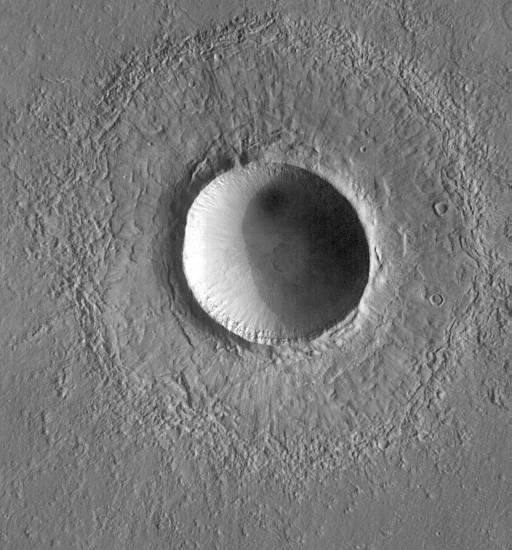
\includegraphics[width=\textwidth,keepaspectratio]{images/Gre13/Gre13_01.jpg}
		\captionsetup{format=plain,width=0.85\textwidth}
		\caption{Eingabebild, aus \cite[Kap.~7]{greeley_13}}
		\label{fig:slic_vs_tsugf_in}
	\end{subfigure}
	\hfill
	\begin{subfigure}[t]{0.32\textwidth}
		\centering
		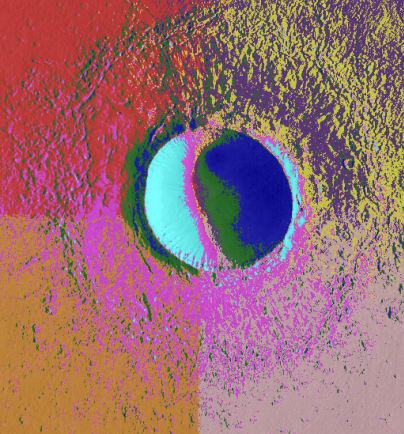
\includegraphics[width=\textwidth,keepaspectratio]{images/gen/slic_vs_tsugf/Gre13_01.jpg_slic.png}
		\captionsetup{format=plain,width=0.85\textwidth}
		\caption{Ergebnis des SLIC-Algorithmus \cite{achanta_10} angewandt auf die Eingabedatei}
		\label{fig:slic_vs_tsugf_slic}
	\end{subfigure}
	\hfill
	\begin{subfigure}[t]{0.32\textwidth}
		\centering
		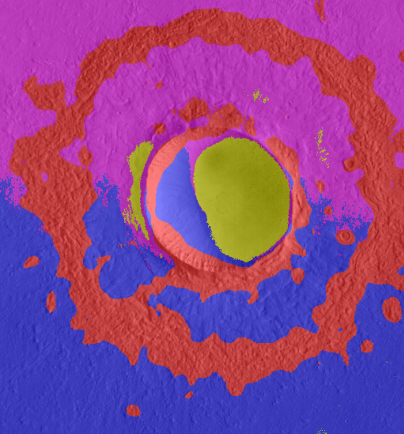
\includegraphics[width=\textwidth,keepaspectratio]{images/gen/slic_vs_tsugf/Gre13_01.jpg_tsugf.png}
		\captionsetup{format=plain,width=0.85\textwidth}
		\caption{Ergebnis des texturbasierten Clusterings (\vgl Unterabschnitt~\ref{ssec:tsugf}) der Eingabedatei}
		\label{fig:slic_vs_tsugf_tsugf}
	\end{subfigure}
	\caption{Clustering eines Graustufenbildes eines Kraters der Marsoberfläche}
\end{figure}

So ergibt ein Clustering des Kraters aus Unterabschnitt~\ref{ssec:mars_surface_features} durch den SLIC-Algorithmus \cite{achanta_10} das in \figurename~\ref{fig:slic_vs_tsugf_slic} sichtbare Ergebnis.\footnote{SLIC-Implementierung: \texttt{scikit-image}\\Parameter: \texttt{compactness=5, n\_segments=10, enforce\_connectivity=False}} Dort ist erkennbar, dass der Krater in jeweilige Licht- und Schattenregionen (bedingt durch den Lichteinfall im flachen Winkel) unterteilt wird. Außerdem wird die raue Struktur ringförmig um den Krater herum schlecht erfasst: An dieser Stelle wird jeder Hügel separat als einerseits helle, andererseits dunkle Stelle markiert. Das Phänomen, dass ein Krater durch eine starke Differenz an Licht- und Schattenregionen erkannt wird wird sich im Großen und Ganzen zwar in Abschnitt~\ref{sec:crater_detection} zu nutze gemacht, ist hier allerdings ungewollt.

Wenn nun der in Unterabschnitt~\ref{ssec:kanezaki} beschriebene Ansatz verfolgt wird, wird das neuronale Netz daraufhin trainiert, eine Aufnahme anhand ihrer Helligkeitsinformationen hin zu trainieren. Da dies nicht gewollt ist, wird statt einem farb-/helligkeitsbasierten Clusteringalgorithmus wie SLIC ein texturbasiertes Clustering genutzt.

Statt des SLIC-Clusterings wird nun die in Unterabschnitt~\ref{ssec:tsugf} vorgestellte Methode des texturbasierten Clusterings genutzt. Von dieser Stelle an sind, wenn nicht anders benannt, die Gewichtungen der verschiedenen Werte für die Farbwerte, X-/Y-Positionen und Reaktion auf Gaborfilter alle gleich $1$. Diese Parameter werden in Unterabschnitt~\ref{ssec:initialization_filterweight} genauer erläutert.

Das Resultat eines Clusterings durch die genutzte, texturbasierte Methode\footnote{Kombiniert mit der Filterbank aus \cite{jain_91}} ist in \figurename~\ref{fig:slic_vs_tsugf_tsugf} sichtbar: Man erkennt, dass der \enquote{Ring} um den eigentlichen Einschlagskrater eine eigenständige Textur besitzt, welche unterschiedlich zu dem Rest der Oberfläche ist. Eine ähnliche Oberflächenstruktur ist direkt um den Krater herum vorhanden. Beide Vorkommnisse dieser ähnlichen Struktur werden vom texturbasierten Clustering erfasst, in ein Segment aufgeteilt und (hier durch eine rote Färbung) markiert.

% TODO Reread

\subsection{Filterbänke}
\label{ssec:initialization_filterbanks}
Nun stellt sich die Frage, welche der vorgestellten Filterbänke sich gut eignet, die Eingabedatei zu clustern. Die größten Unterschiede zwischen den einzelnen Filterbänken besteht darin, dass einige von ihnen rotationsinvariante Filter enthalten, und andere in mehreren Größen vorhanden sind. Die Größendifferenz lässt sich in der Anwendung des Algorithmus dadurch ausgleichen, dass jeder Filter zusätzlich in weitere Größen skaliert wird, und in jeder Skalierungsstufe angewandt wird. Die Rotationsinvarianz würde sich höchstens durch die Rotation der Filter approximieren lassen, da so allerdings nicht jeder Winkel abgedeckt werden kann, ist diese Methode ungeeignet. In \figurename~\ref{fig:filterbank_comparision} ist die Anwendung der in Unterabschnitt~\ref{ssec:tsugf} vorgestellten Filterbänke auf vier Beispielbilder (\vgl Abschnitt~\ref{ssec:mars_surface_features}) sichtbar. Diese sind nach deren Bezeichnungen in genanntem Abschnitt benannt. Jedes Bild wurde in vier Cluster aufgeteilt und alle Optimierungen des Verfahrens (\vgl Unterabschnitt~\ref{ssec:tsugf}) wurden angewandt.

\paragraph{Krater}
Neben dem eigentlichen Krater ist auf dieser Aufnahme der Ring aus gröberem Gestein ein wichtiges Merkmal. Dieser wird von allen Filterbänken zuverlässig erkannt, wenn auch mit einer unterschiedlichen Dicke: Die LM- und S-Filterbank selektieren dieses Gestein eher großzügig, die MR-Filterbank hingegen zeigt sehr enge Markierungen dieser Region.

Alle Filterbänke formen einen Ring (oder dessen Ansatz) auf dem Kraterrand, die Maximum Response-Filterbank erzeugt zwei konzentrische Ringe

Der Krater selbst wird von den Filterkombinationen nach \cite{jain_91} und der LM-Filterbank leider nur in Hell- und Dunkel-Regionen aufgeteilt, die S-Filterbank zeigt innerhalb des Kraters kein brauchbares Ergebnis. Eine Ausnahme stellt die Maximum-Response-Filterbank dar, welche neben den zwei erwähnten konzentrischen Clustern den Bereich innerhalb des Kraters als ein einziges Cluster erkennt. Die Maximum Response-Bank erzeugt in diesem Bereich das Resultat, welches sich wohl als bestes zur Weiterverarbeitung eignet.

% TODO Weil...

\paragraph{Vulkan}
Der Vulkanberg wird leider von keiner Filterbank optimal erkannt. Der äußere Rand wird nur von der S-Filterbank als ein Cluster erkannt, dies allerdings nicht sehr genau. Der rauere Bereich der Oberfläche, was kleinere Krater miteinbeschließt, wird vom MR-Filter am ehesten und genausten erkannt, auf dem zweiten Platz folgt die Filterbank nach \cite{jain_91}, welche zwar alle Krater in ein Cluster fügt (violett), allerdings eher gröber.

Die Vulkanmitte wird von keiner Filterbank erkannt, nur bei der MR-Bank lässt sich eine ringförmige, rauere Stelle um den Krater herum erahnen. Die anderen Filterbänke selektieren an dieser Stelle hauptsächlich nach den Helligkeitswerten. Außerdem ist interessant, dass der LM-Filter die Bergspitzen in vom Umfeld getrennte Cluster einteilt (blau und violett). Somit scheint es, als ließe sich diese Aufnahme über keine Filterbank gut clustern. Am ehesten eignet sich allerdings erneut die MR-Bank.

\paragraph{Vulkan mit strahlenförmigen Merkmalen}

Das Ziel bei der Nutzung dieser Marsaufnahme zur Analyse besteht daraus zu analysieren, mit welcher Filterbank die konzentrischen Strahlen am genauesten erkannt werden. Des Weiteren existieren auf der Aufnahme noch Krater, welche es separat einzuordnen gilt.

Die Filterbank nach \cite{jain_91} erkennt die gröberen Strukturen (Strahlen und Krater), fügt diese allerdings in dasselbe Cluster ein (gelb und blau).

Die LM-Filterbank scheint kein brauchbares Ergebnis zu produzieren, sie erkennt im Allgemeinen nur einige der Krater (rot) separat von deren Umfeld, die Strahlen sind nicht geeignet geclustert worden.

Die Schmid-Filterbank clustert einen Großteil der Strahlen gemeinsam in ein Cluster (rot). Die Krater hingegen sind nicht fest einer Clusterart zugewiesen, ein Großteil von ihnen befindet sich jedoch auch im roten Cluster.

Wie in den vorherigen Tests ist das Resultat der MR-Filterbank schon fast zu genau, die Cluster sind sehr fein gehalten. Im Gegensatz zu den Alternativen, werden hier die Krater relativ zuverlässig in gelbe Cluster eingeordnet, die Strahlen sind leider zu fein markiert, als dass man sie getrennt erkennen könnte. Dieses Phänomen könnte sich allerdings in der praktischen Anwendung zunutze gemacht werden, da dafür eine zu feine Initialisierung notwendig ist.

\paragraph{Gletscher}

Der Gletscher stellt im Bereich der Bildsegmentierung ein vergleichsweise schwieriges Problem dar, da er an vielen seiner Ränder keine feste Grenze zu benachbarten Regionen zeigt, nur links auf der Aufnahme ist er durch eine Hügelreihe strikt begrenzt. Diese Grenze wird von allen Filterbänken in ein getrenntes Cluster unterteilt,mit Ausnahme der Filterbank nach \cite{jain_91}: Diese produziert kein geeignetes Ergebnis, nur die stärker erkennbaren \enquote{Streifen} werden gut erkannt (violett). Die LM-Filterbank erkennt zwar die Abgrenzung auf der linken Seite, allerdings keine anderen Regionen korrekt. Sie liefert bei diesem Bild das wohl schlechteste Resultat. Die Maximum-Response Methode und die Filterbank nach \cite{schmid_01} liefern zwar etwas bessere Ergebnisse, diese sind allerdings nicht gut. Die MR-Bank erzeugt erneut sehr feine Cluster.

\paragraph{}
Zusammengefasst erzeugt aus dieser Auswahl an Filterbänden die Maximum Response-Methode von \cite{visgeo} das wohl am ehesten geeignete Resultat zur Weiterverarbeitung. Auf zweitem Platz folgt die Schmid-Filterbank.

\begin{figure}[h!]
\setlength\tabcolsep{1pt}
\def\arraystretch{0.5}
\begin{tabular}{p{0.2\textwidth}p{0.2\textwidth}p{0.2\textwidth}p{0.2\textwidth}p{0.2\textwidth}}
	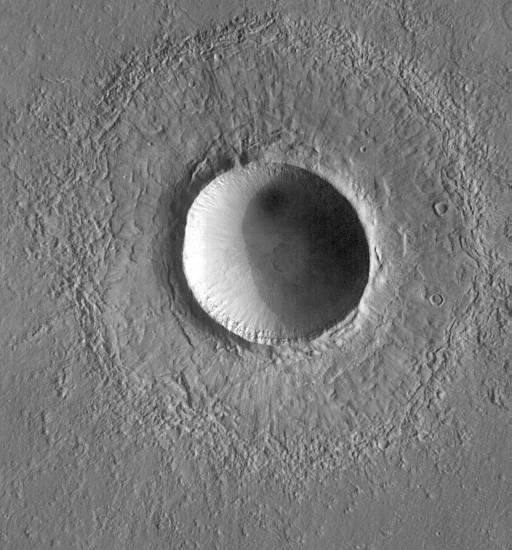
\includegraphics[width=0.2\textwidth]{images/Gre13/Gre13_01.jpg} &
	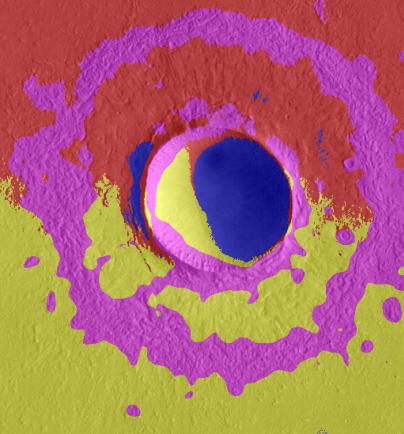
\includegraphics[width=0.2\textwidth]{images/gen/filterbanks/Gre13_01.jpg_TSUGF.png} &
	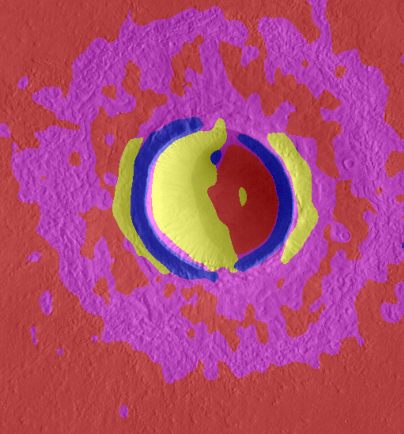
\includegraphics[width=0.2\textwidth]{images/gen/filterbanks/Gre13_01.jpg_LM.png} &
	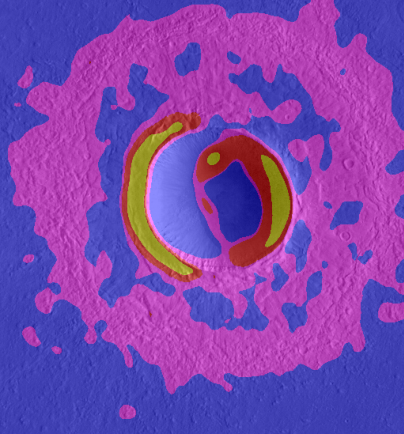
\includegraphics[width=0.2\textwidth]{images/gen/filterbanks/Gre13_01.jpg_S.png} &
	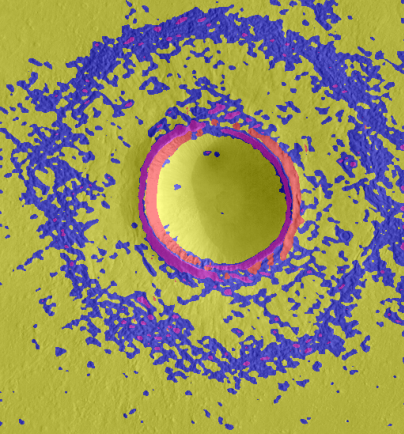
\includegraphics[width=0.2\textwidth]{images/gen/filterbanks/Gre13_01.jpg_MR.png} \\
	
	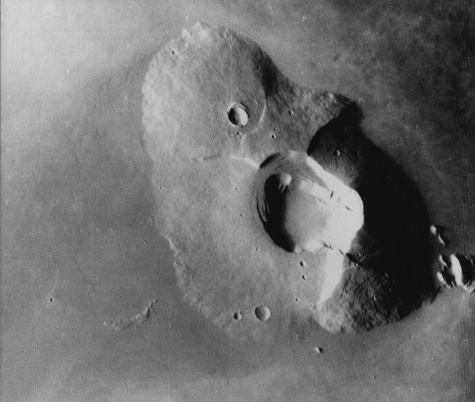
\includegraphics[width=0.2\textwidth]{images/Gre13/Gre13_02.jpg} &
	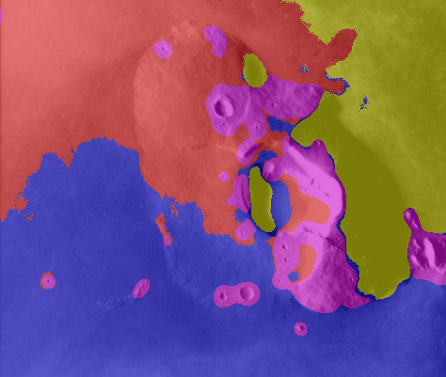
\includegraphics[width=0.2\textwidth]{images/gen/filterbanks/Gre13_02.jpg_TSUGF.png} &
	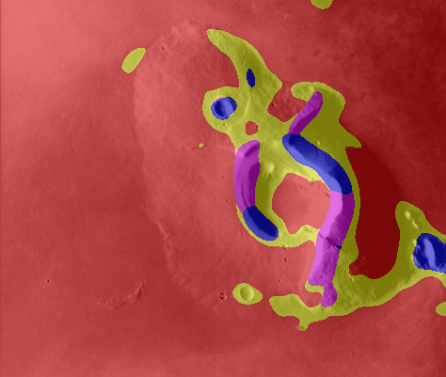
\includegraphics[width=0.2\textwidth]{images/gen/filterbanks/Gre13_02.jpg_LM.png} &
	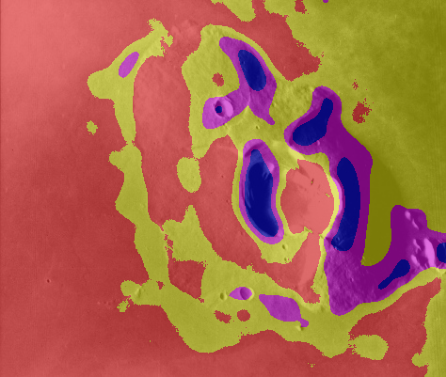
\includegraphics[width=0.2\textwidth]{images/gen/filterbanks/Gre13_02.jpg_S.png} &
	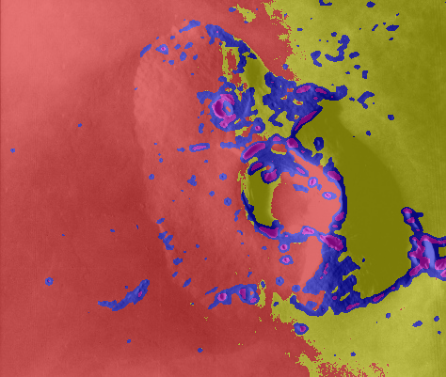
\includegraphics[width=0.2\textwidth]{images/gen/filterbanks/Gre13_02.jpg_MR.png} \\
	
	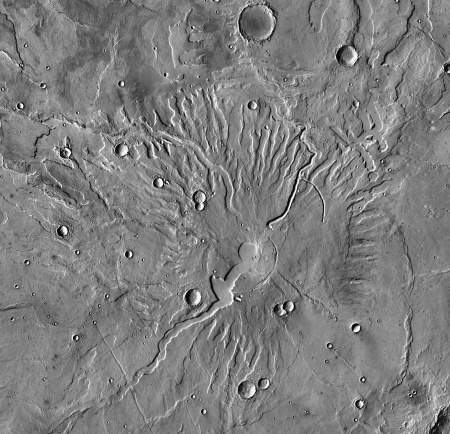
\includegraphics[width=0.2\textwidth]{images/Gre13/Gre13_03.jpg} &
	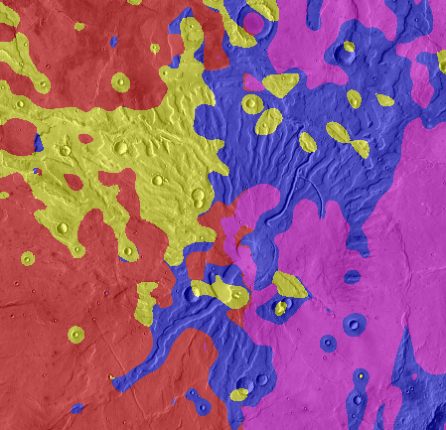
\includegraphics[width=0.2\textwidth]{images/gen/filterbanks/Gre13_03.jpg_TSUGF.png} &
	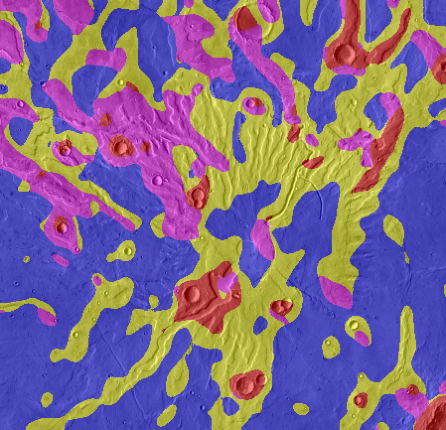
\includegraphics[width=0.2\textwidth]{images/gen/filterbanks/Gre13_03.jpg_LM.png} &
	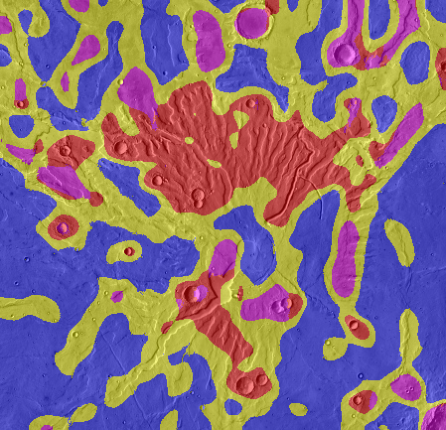
\includegraphics[width=0.2\textwidth]{images/gen/filterbanks/Gre13_03.jpg_S.png} &
	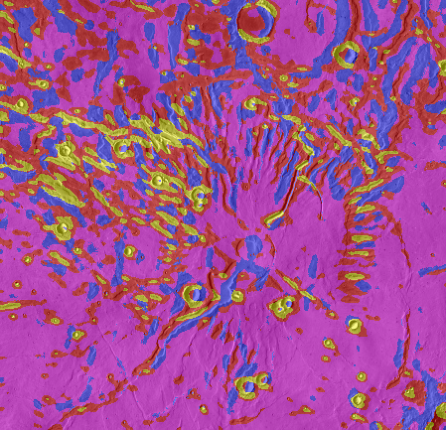
\includegraphics[width=0.2\textwidth]{images/gen/filterbanks/Gre13_03.jpg_MR.png} \\
	
	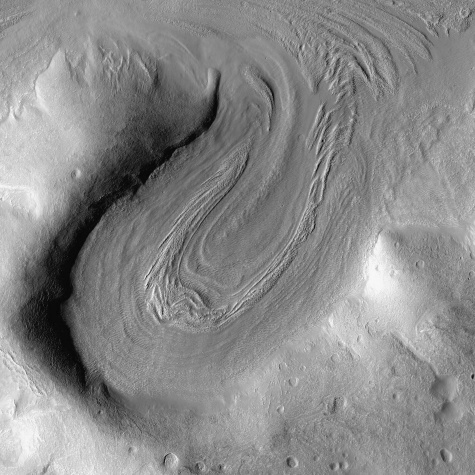
\includegraphics[width=0.2\textwidth]{images/Gre13/Gre13_05.jpg} &
	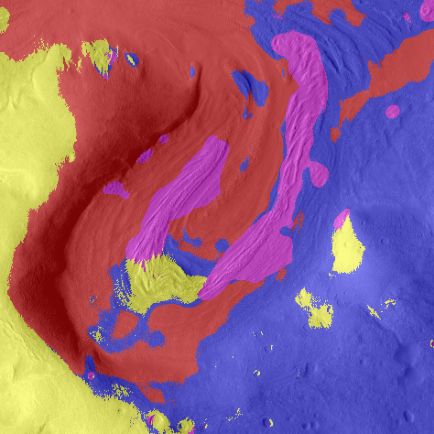
\includegraphics[width=0.2\textwidth]{images/gen/filterbanks/Gre13_05.jpg_TSUGF.png} &
	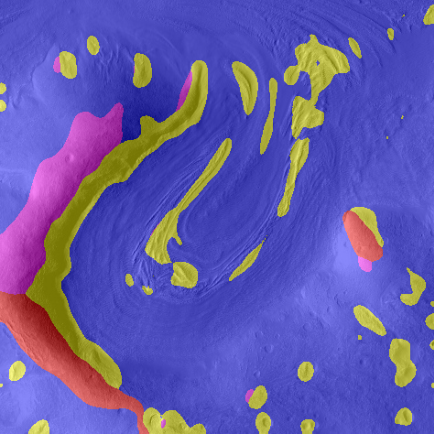
\includegraphics[width=0.2\textwidth]{images/gen/filterbanks/Gre13_05.jpg_LM.png} &
	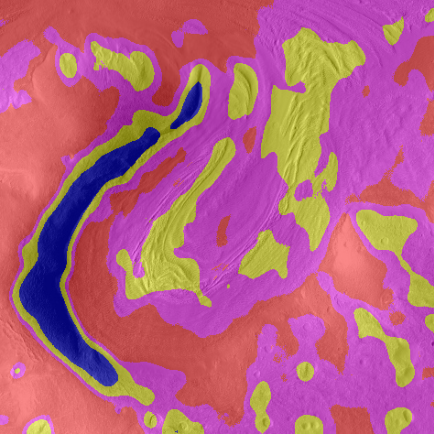
\includegraphics[width=0.2\textwidth]{images/gen/filterbanks/Gre13_05.jpg_S.png} &
	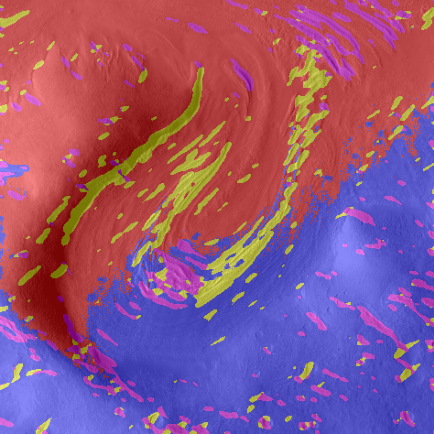
\includegraphics[width=0.2\textwidth]{images/gen/filterbanks/Gre13_05.jpg_MR.png} \\
	
	\hspace{1pt}\newline\centering Eingabe, aus \cite{greeley_13} &
	\hspace{1pt}\newline\centering Filterbank nach \cite{jain_91} &
	\hspace{1pt}\newline\centering LM-Filterbank \cite{leung_01} &
	\hspace{1pt}\newline\centering S-Filterbank \cite{schmid_01} &
	\hspace{1pt}\newline\centering MR-Filterbank \cite{visgeo} \\
\end{tabular}
\caption{Vergleich verschiedener Filterbänke auf Bildern der Marsoberfläche (Krater, Vulkan, Vulkan mit strahlenförmigen Merkmalen, Gletscher). Die Farben der jeweiligen Cluster wurden zufällig gewählt und sagen nichts über deren Inhalt aus. Alle Bilder wurden in vier Cluster eingeteilt.}
\label{fig:filterbank_comparision}
\end{figure}

\subsection{Größe der Filter}
\label{ssec:initialization_filtersize}

Neben der Auswahl einer geeigneten Filterbank lassen sich in dieser noch die einzelnen Gewichtungen anpassen: So könnten \zB die Gewichtung der Koordinaten der Pixel zueinander oder die Relevanz von ähnlichen Farbwerten modifiziert werden. Außerdem ist die Größe der einzelnen Filter in den jeweiligen Filterbänken auch Variabel und muss dementsprechend an die Dimensionen des jeweiligen Eingabebildes angepasst werden. Da alle Filterbänke (bis auf die nach \cite{jain_91}) jeweils gleiche Filter in unterschiedlichen Größen enthalten, muss nur ein Gesamtwert angepasst werden, statt der Größe jeder einzelnen Skalierung. Es wird nun versucht, die Ergebnisse der Maximum Response-Filterbank zu verbessern, da diese in vorherigen Versuchen die besten Ergebnisse erzielt hat.

Von dieser Stelle an müssen Marsaufnahmen genutzt werden, bei denen die Auflösung bekannt ist, somit scheiden die bis hierhin genutzten Aufnahmen aus \cite{greeley_13} leider aus. Stattdessen werden Ausschnitte aus der Aufnahme \texttt{P03\_002147\_1865\_XI\_06N208W} der Context Camera des Mars Reconnaissance Orbiters genutzt. Ein weiterer Vorteil der Nutzung dieser Bilder besteht daraus, dass die Clusteringalgorithmen nun an realitätsnähreren Daten getestet werden können, statt an isolierten Aufnahmen einzelner Besonderheiten der Oberfläche. Die Ergebnisse sind in \figurename~\ref{fig:filterbank_sizes} zu sehen. Als Startwert wurde ein Skalierungsfaktor $s=1$ betrachtet, angewandt auf die vorgestellten, quadratischen Filter mit einer originalen Kantenlänge von \SI{49}{\pixel}. Dieser wurde nach oben und unten hin in Schritten von $\Delta s=0.25$ verändert, und mit der skalierten MR-Filterbank ein neues Clustering der vier Ausschnitte erstellt. Die Eingabebilder sind quadratisch und besitzen eine Seitenlänge von \SI{650}{\pixel} bei einer Auflösung von \SI{6,17}{\meter\per\pixel}. Jedes der Eingabebilder wurde erneut in vier Bereiche eingeteilt, die Farben sind zur Veranschaulichung zufällig gewählt.

\paragraph{Skalierungsfaktor $s=0,25$}

Auf der ersten Aufnahme ist, vergleichbar mit den Beispielaufnahmen aus dem letzten Abschnitt, ein runder Krater zentriert zu sehen. Die geringe Skalierung mit dem Faktor $s=0.25$ führt dazu, dass die jeweiligen Filter zu klein sind, um die Strukturen der Oberfläche zu erkennen, somit sieht diese Aufnahme aus, als wäre nur anhand ihrer Helligkeitswerten geclustert worden. Das gleiche gilt auch für die zweite und vierte Aufnahme.

Die dritte Aufnahme stellt eine relativ ebenmäßige Fläche in einem Umfeld von gröberer Oberfläche dar. Dort scheint es, als gäbe es nicht genug Kontrast um nach den Helligkeitswerten zu clustern, der Algorithmus erstellt eine Filterung anhand der X- und Y-Koordinaten. Bei allen Aufnahmen werden nur zwei wirkliche Cluster erstellt, die letzten zwei Cluster die erstellt werden sollten bestehen nur aus jeweils wenigen Pixeln.

Dieser Skalierungsfaktor produziert keine brauchbaren Ergebnisse.

\paragraph{Skalierungsfaktor $s=0,50$}

Wie zu erwarten führt die genutzte, noch relativ geringe Skalierung der Filterbank mit $s=0,50$ zu vielen kleineren Clustern, in diesem Fall auf der ersten Aufnahme deutlich erkennbar anhand der gelb markierten Flächen. Obwohl es auf den ersten Blick scheint, als würden die Kraterränder erkannt werden, werden durch die Filterbank bei dieser Skalierung nur die dunkleren Bereiche, in diesem Fall die Schatten, die die erhöhten Kraterränder werfen, erkannt. Auf dieser Aufnahme führt dies zwar zu einer vergleichsweise guten Approxmimation der Krater, sobald anderweitige Schatten hinzukommen, wird diese Skalierung allerdings keine geeigneten Resultate produzieren.

Das selbe Phänomen tritt bei der zweiten Aufnahme auf, auch dort wird stark anhand der Helligkeitswerte geclustert, erkennbar insbesondere an den violetten Bereichen an den Kraterrändern. Bei diesem Bild wird allerdings auch trotz der kleineren Skalierung das raue Gebiet, welches sich horizontal durch das Bild erstreckt, in ein (rot gefärbtes) Cluster eingeteilt. Auch hier werden allerdings dunklerere Bereiche (wie die Kraterränder) in separate (violett gefärbte) Cluster eingeteilt.

Auf der dritten Aufnahme wird bei der genutzten Skalierung die feinere Fläche größtenteils als ein (gelb gefärbtes) Cluster dargestellt, separat dazu sind in rot die Übergänge zwischen den Regionen gekennzeichnet. Die gröberen Flächen in den äußeren Bereichen werden nicht zuverlässig in das selbe Cluster eingeordnet.

Die letzte Testaufnahme, bestehend aus zwei Hügeln \bzw Bergen, stellt durch die über- und unterbelichteten Flächen an den Hängen eine der größten Herausforderungen für den Clusteringalgorithmus dar. An diesen Stellen ist der Kontrast des Bildes sehr gering, sodass kaum noch Texturen erkannt werden, anhand derer geclustert werden könnte. Wie zu erwarten werden die dunklen Flächen in ein einzelnes (rotes) Cluster kombiniert. Kleine Hügelketten hingegen werden zuverlässig in zusammengehörige Cluster eingeteilt, welches auf diesen Aufnahmen blau markiert ist. Die beleuchteten Seiten der Hügel werden bei dieser Skalierung leider nicht von der allgemeinen Marsoberfläche unterschieden, höchstens der Fuß des Berges kann durch die violette Färbung erahnt werden.

Dieser Skalierungsfaktor führt zu vergleichsweise guten Clusteringergebnissen.

\paragraph{Skalierungsfaktor $s=0,75$}

Dieser Skalierungsfaktor führt beim Clustering des ersten Bildes zu Resultat, welche vergleichbar mit denen des Faktors $s=0,5$ sind. Die Ränder der Krater werden allerdings getrennt in helle und dunkle Regionen eingeteilt, die Cluster im äußeren Bereich sind größer und gröber.

Auf der zweiten Aufnahme wird die horizontale rauere Region sehr gut in ein eigenes Cluster eingeteilt, selbiges gilt für die Kraterränder. Auf dieser Aufnahme erscheint der Skalierungsfaktor $s=0,75$ für diese Filterbank optimal.

Die dritte Aufnahme unterscheidet sich bis auf die gröberen, größeren Cluster in den äußeren Bereichen nicht wesentlich von der vorherigen Skalierung.

Bei der letzten Aufnahme führt die größere Skalierung zu einem uniformen Clusterings des beleuchteten Berghangs, er wird als eine große Fläche erkannt. Die dunkle Seite hingegen wird in zwei Cluster unterteilt: Die eigentliche dunkle Seite des Berges, und die Stellen, welche zu unterbelichtet sind, um aus ihnen eine Textur zu erkennen.

Insgesamt scheint sich dieser Skalierungsfaktor auch zum textutbasierten Clustering zu eignen.

\paragraph{Skalierungsfaktor $s=1.00$}

Während bei diesem Skalierungsfaktor auf der ersten Aufnahme der größere, mittige Krater relativ gut durch ein gelbes kreisförmiges Cluster gekennzeichnet wird, wird der kleinere Krater nicht zuverlässig erkannt. Bei diesem gehen die Cluster in umlegende Gebiete über, als wäre dieser Krater nur eine etwas rauere Oberflächenstruktur.

Bei der zweiten Aufnahme wird wie zuvor der Krater erfolgreich separat in ein Cluster eingeteilt, die Begrenzungen der gröberen Struktur, welche sich durch das Bild zieht, geht allerdings verloren. Diese Region wird leider im rechten Teil des Bildes sehr weitläufig erkannt.

In dem dritten Testbild werden die gröberen Hügelketten am Rand des helleren Bereiches zwar erkannt (gelb markiert), und die Übergangsstellen zwischen zwei Regionen werden in ein blaues Cluster zusammengefügt, alle anderen Regionen sind allerdings nicht voneinander getrennt worden.

Das letzte Bild wird bei dieser Skalierung fast identisch zu der Skalierung mit $s=0,75$ geclustert.

Zusammengefasst ist diese Skalierung schon zu grob um so gute Ergebnisse wie die vorherigen zu erreichen.

\paragraph{Skalierungsfaktor $s=1.25$ und $s=1.50$}

Da diese beiden Skalierungsfaktoren zu fast identischen Clusterverteilungen führen, werden sie in einen Abschnitt zusammengefasst.

Bei diesen Skalierungen werden im oberen, glätteren Bereich der ersten Aufnahme die vereinzelten Krater wie gewollt erkannt, sie versagt allerdings im unteren, gröberen Bereich, wo sie nur ein großes Cluster erstellen. Der Krater wird nur anhand von starken Helligkeitsdifferenzen erkannt, welche in der gesamten Ausgabe gelb bei $s=1,25$, \bzw violett bei $s=1,5$ markiert wurden. 

Selbiges gilt im Bezug auf die starken Helligkeitsdifferenzen bei der zweiten Aufnahme.

Bei der dritten Aufnahme wird von beiden Skalierungsfaktoren kein brauchbares Resultat produziert, man kann höchstens erahnen, dass die gelb \bzw violett gefärbten Regionen besonders kontrastarme, also glatte Flächen darstellen sollen.

Beim Clusteringergebnis der letzten Aufnahme unterschieden sich die beiden Skalierungsfaktoren erstmals stärker: Bei $s=1,25$ gleicht das Ergebnis dem des vorherigen Clusterings: Kleinere Bergregionen und rauere Oberflächenstrukturen werden getrennt voneinander erkannt, Flächen mit weniger oder (aufgrund von Unterbelichtung) keiner werden auch in ein großes Cluster hinzugefügt. Der Faktor $s=1,5$ scheint selbst bei diesem Bild zu groß zu sein, bis auf die Hügelketten mit starker Helligkeitsdifferenz wird die Aufnahme nur anhand ihrer Helligkeitswerte geclustert.

Diese Faktoren sind also zu groß um brauchbare Resultate zu produzieren.

\begin{figure}[h!]
	\setlength\tabcolsep{1pt}
	\def\arraystretch{0.5}
	\begin{tabular}{C{0.14\textwidth}C{0.14\textwidth}C{0.14\textwidth}C{0.14\textwidth}C{0.14\textwidth}C{0.14\textwidth}C{0.14\textwidth}}
		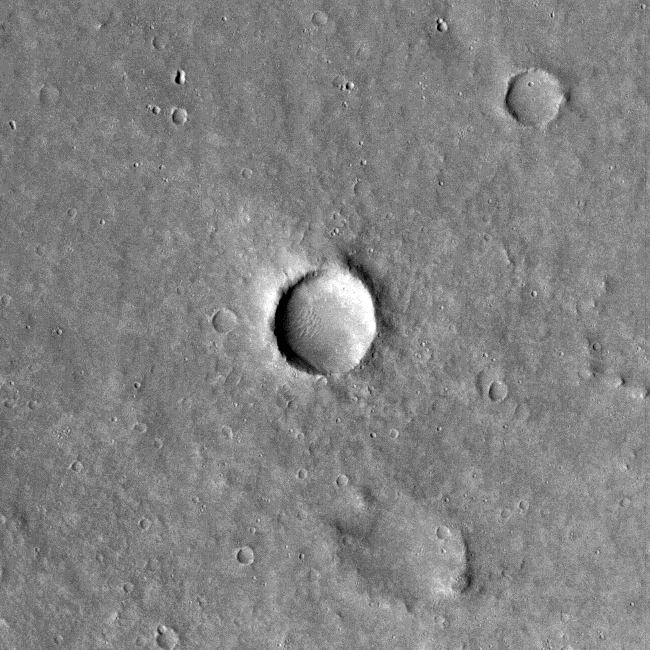
\includegraphics[width=0.14\textwidth]{images/p03/p03_01.png} &
		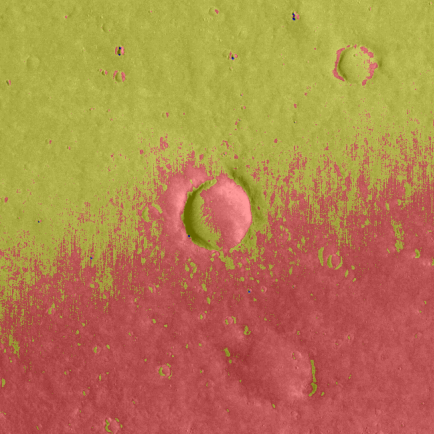
\includegraphics[width=0.14\textwidth]{images/gen/filter_size/p03_01.png_0.25.png} &
		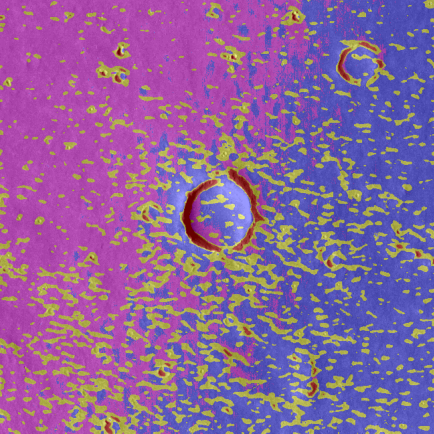
\includegraphics[width=0.14\textwidth]{images/gen/filter_size/p03_01.png_0.50.png} &
		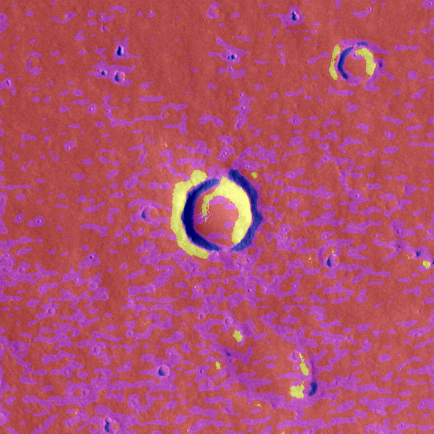
\includegraphics[width=0.14\textwidth]{images/gen/filter_size/p03_01.png_0.75.png} &
		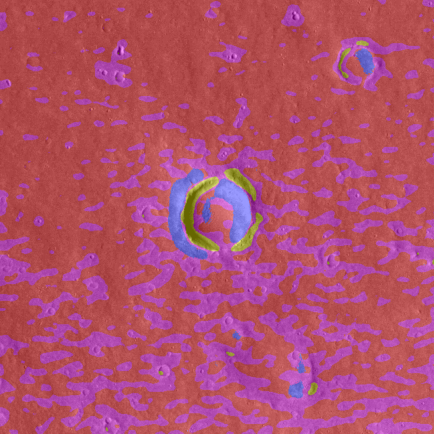
\includegraphics[width=0.14\textwidth]{images/gen/filter_size/p03_01.png_1.00.png} &
		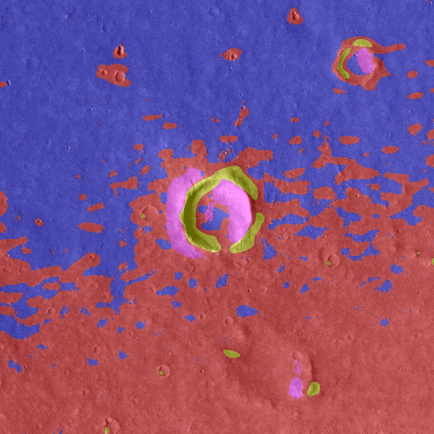
\includegraphics[width=0.14\textwidth]{images/gen/filter_size/p03_01.png_1.25.png} &
		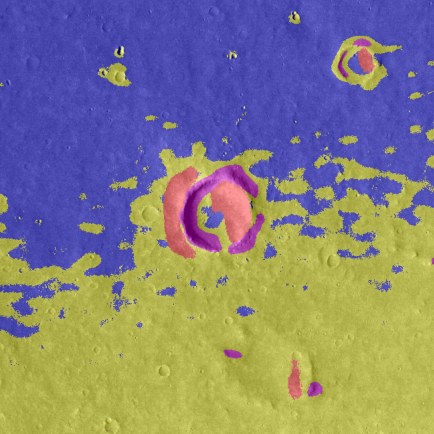
\includegraphics[width=0.14\textwidth]{images/gen/filter_size/p03_01.png_1.50.png} \\
		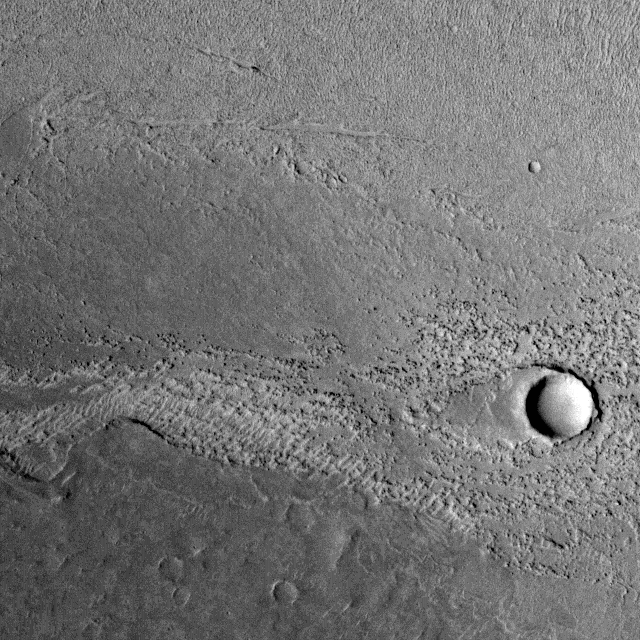
\includegraphics[width=0.14\textwidth]{images/p03/p03_02.png} &
		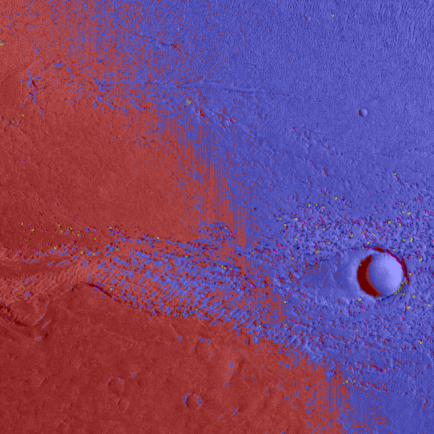
\includegraphics[width=0.14\textwidth]{images/gen/filter_size/p03_02.png_0.25.png} &
		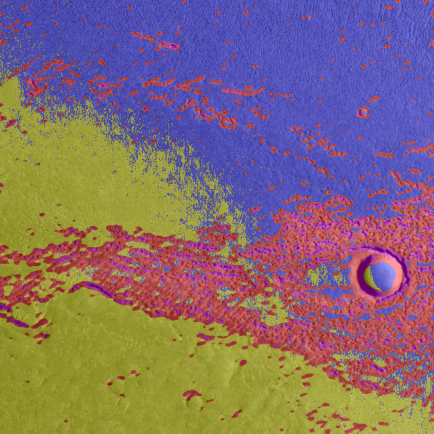
\includegraphics[width=0.14\textwidth]{images/gen/filter_size/p03_02.png_0.50.png} &
		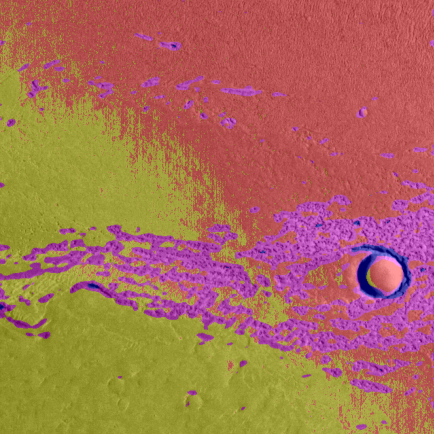
\includegraphics[width=0.14\textwidth]{images/gen/filter_size/p03_02.png_0.75.png} &
		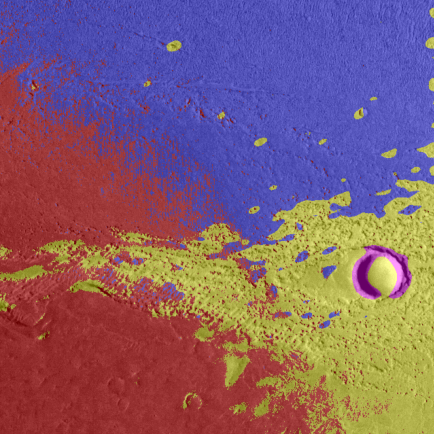
\includegraphics[width=0.14\textwidth]{images/gen/filter_size/p03_02.png_1.00.png} &
		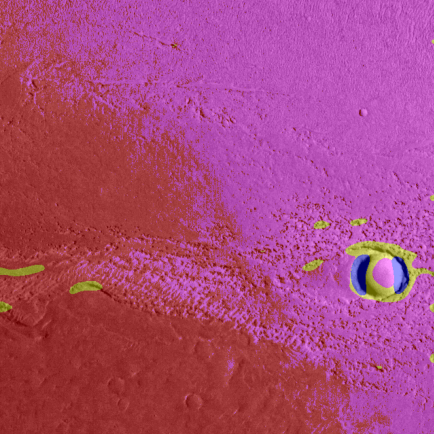
\includegraphics[width=0.14\textwidth]{images/gen/filter_size/p03_02.png_1.25.png} &
		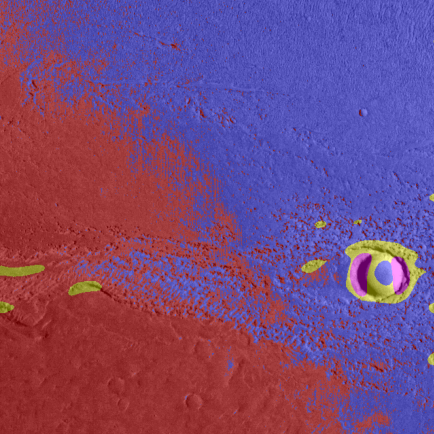
\includegraphics[width=0.14\textwidth]{images/gen/filter_size/p03_02.png_1.50.png} \\
		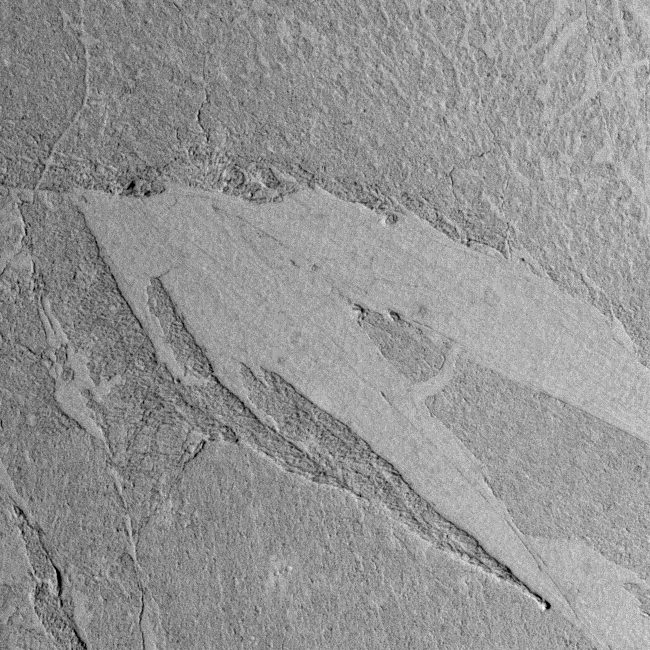
\includegraphics[width=0.14\textwidth]{images/p03/p03_03.png} &
		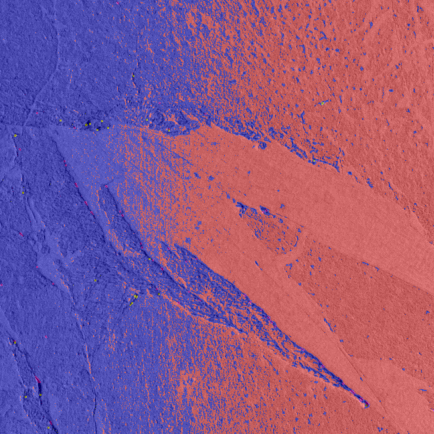
\includegraphics[width=0.14\textwidth]{images/gen/filter_size/p03_03.png_0.25.png} &
		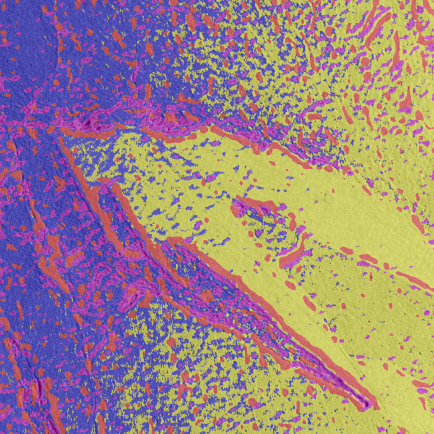
\includegraphics[width=0.14\textwidth]{images/gen/filter_size/p03_03.png_0.50.png} &
		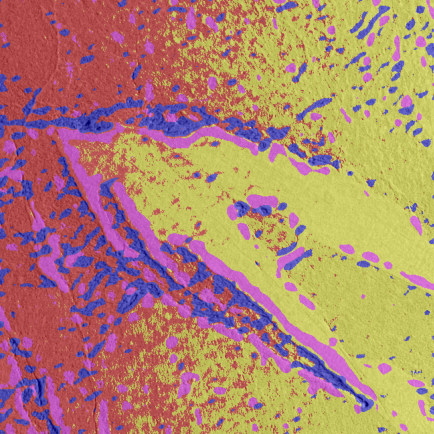
\includegraphics[width=0.14\textwidth]{images/gen/filter_size/p03_03.png_0.75.png} &
		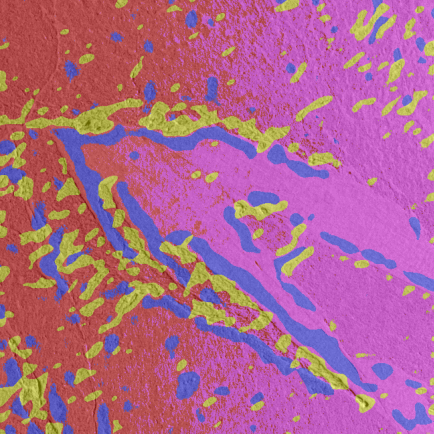
\includegraphics[width=0.14\textwidth]{images/gen/filter_size/p03_03.png_1.00.png} &
		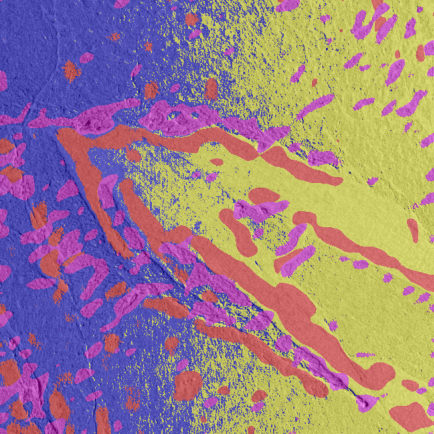
\includegraphics[width=0.14\textwidth]{images/gen/filter_size/p03_03.png_1.25.png} &
		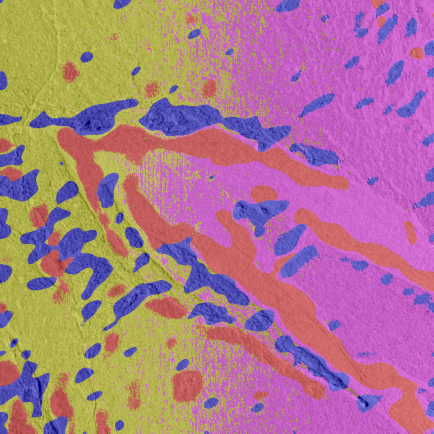
\includegraphics[width=0.14\textwidth]{images/gen/filter_size/p03_03.png_1.50.png} \\
		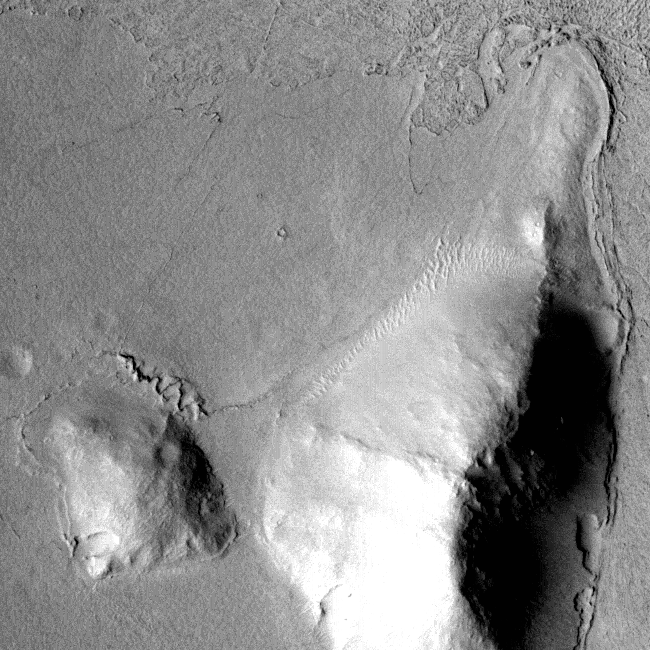
\includegraphics[width=0.14\textwidth]{images/p03/p03_04.png} &
		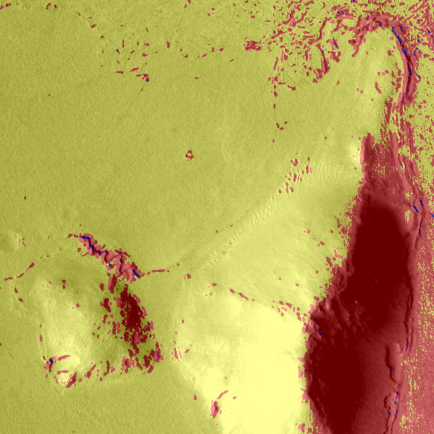
\includegraphics[width=0.14\textwidth]{images/gen/filter_size/p03_04.png_0.25.png} &
		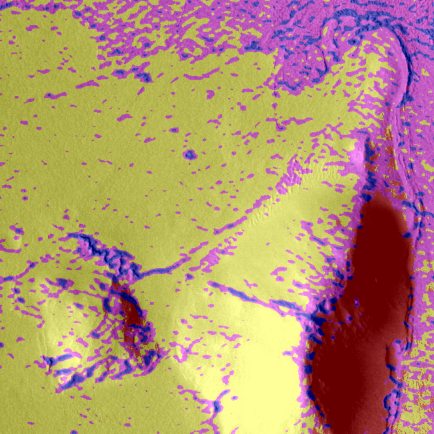
\includegraphics[width=0.14\textwidth]{images/gen/filter_size/p03_04.png_0.50.png} &
		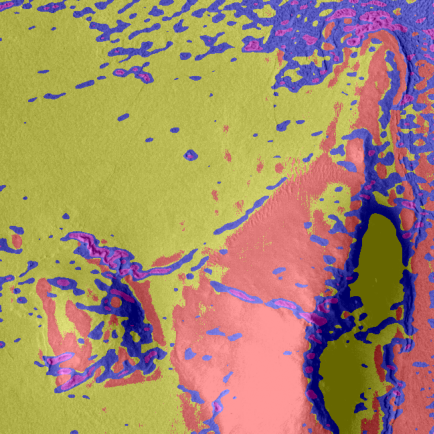
\includegraphics[width=0.14\textwidth]{images/gen/filter_size/p03_04.png_0.75.png} &
		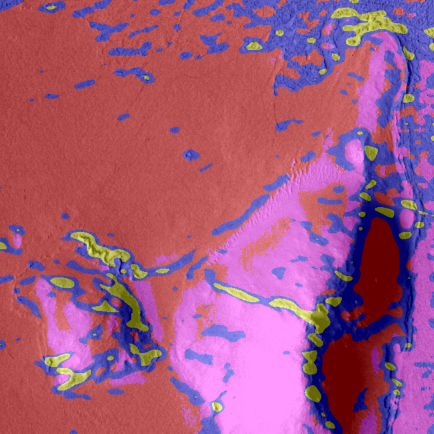
\includegraphics[width=0.14\textwidth]{images/gen/filter_size/p03_04.png_1.00.png} &
		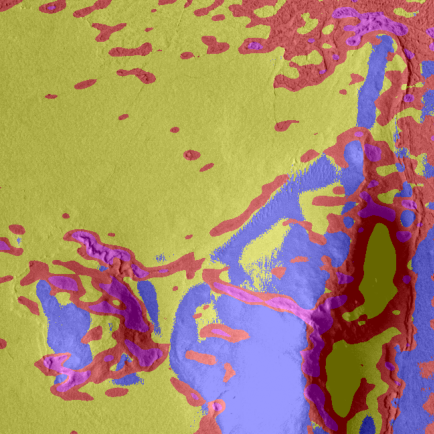
\includegraphics[width=0.14\textwidth]{images/gen/filter_size/p03_04.png_1.25.png} &
		\includegraphics[width=0.14\textwidth]{images/gen/filter_size/p03_04.png_1.50.png} \\
		
		\hspace{2pt}\newline\centering Eingabe & 
		\hspace{2pt}\newline\centering $s=0,25$ &
		\hspace{2pt}\newline\centering $s=0,50$ &
		\hspace{2pt}\newline\centering $s=0,75$ &
		\hspace{2pt}\newline\centering $s=1,00$ &
		\hspace{2pt}\newline\centering $s=1,25$ &
		\hspace{2pt}\newline\centering $s=1,50$
	\end{tabular}
	\caption{Vergleich verschiedener Skalierungen der MR-Filterbank auf Bildern der Marsoberfläche. Die Farben der jeweiligen Cluster wurden zufällig gewählt und sagen nichts über deren Inhalt aus. Alle Bilder wurden in vier Cluster eingeteilt.}
	\label{fig:filterbank_sizes}
\end{figure}

\paragraph{}
Aus diesen Ergebnissen lässt sich schlussfolgern, dass sich die Skalierungsfaktoren $s=0,5$ und $s=0,75$ bei diesen Eingabedaten die besten Resultate liefert. Da durch die nachfolgende Weiterverarbeitung durch den Algorithmus nach Kanezaki eine hohe Anzahl an Clustern benötigt wird, diese aber nicht zu klein und Verstreut ausfallen sollten, wird von nun an ein Skalierungsfaktor von $s=0,75$ genutzt.

\subsection{Gewichtungen der Parameter}
\label{ssec:initialization_filterweight}

Da in dem Prozess des Clusterings alle Optimierungen aus Unterabschnitt~\ref{ssec:tsugf} miteingeschlossen sind, beinhaltet dies, dass der Datenwürfel, den k-Means verarbeitet, sowohl die Koordinaten, als auch die Farbwerte der Eingabedatei beinhaltet. Nun stellt sich die Frage, wie stark diese jeweils gewichtet werden sollten, um ein akzeptables Ergebnis zu erhalten. Aus diesem Grund sind in den Abbildungen~\ref{fig:filterbank_weights_pos} und \ref{fig:filterbank_weights_col} die Resultate des Clusterings mit unterschiedlichen Werten für die jeweiligen Gewichtungen zu sehen. Die Skalierung der Filter beträgt $s=0,5$, da im vorherigen Unterabschnitt festgestellt wurde, dass dieser Wert relativ gute Ergebnisse liefert.

\paragraph{Gewichtung der Koordinaten}
Das Hinzufügen der X- und Y-Koordinaten zu dem Datenwürfel ist ursprünglich aus dem Grund geschehen, dass ein gegebener räumlicher Bezug zwischen unterschiedlichen Pixeln beim Clustering berücksichtigt werden kann (\vgl Unterabschnitt~\ref{ssec:tsugf}; \cite{jain_91}). Aus den Clusteringergebnissen in \figurename~\ref{fig:filterbank_weights_pos} allerdings lässt sich erkennen, dass dieser räumliche Bezug in diesem Anwendungsfall nicht außerordentlich hilfreich ist: Bei einer Gewichtung von $w_p\geq1,33$ lässt sich eindeutig erkennen, dass der allgemeine Bodenbereich auf allen Aufnahmen zu stark Anhand seiner Positionen eingeteilt wird, es entstehen Cluster in den Ecken der Aufnahmen, welche sich ins Zentrum erstrecken. Unter diesem starken Einfluss nimmt zusätzlich die relative Wichtigkeit der ähnlichen Textur ab.

Wird nun ein geringerer Wert für $w_p$ betrachtet, so erkennt man für Werte mit $w_p\leq0.66$ keinen Starken Unterschied bei wechselnden Gewichtungen. Dies ist insbesondere bei $w_p=0$ signifikant, da dort der räumliche Bezug der einzelnen Pixel zueinander bei der Berechnung des Clusterings zwar komplett ignoriert wird, das eigentliche Ergebnis sich --~bis auf etwas kleinere Cluster in den merkmalsarmen Bereichen~-- aber kaum verändert. Dies lässt sich darauf zurückführen, dass das Hinzufügen des räumlichen Bezuges ursprünglich den Grund hatte, dass auf \enquote{normalen} Fotografien die vorkommenden Cluster meistens nur ein einziges mal an einem räumlich begrenzten Ort vorhanden sind, so sind \zB bei der Aufnahme aus \figurename~\ref{fig:tsugf_optim} aus Unterabschnitt~\ref{ssec:tsugf} die kleineren Korallen im linken Hintergrund nur an dieser Stelle vorhanden und ließen sich durch ein weit ausgedehntes Cluster zusammenfassen. Bei den aktuell genutzten Aufnahmen hingegen ist dies nicht der Fall, eine auftretende Oberflächenstruktur, wie \zB ein Krater kann an verschieden Stellen ohne räumlichen Bezug zueinander auftreten.
Die Nutzung der Positionwerte hat allerdings einen Vorteil: Sie sorgt dafür die Clustergrößen nicht zu klein und fragmentiert werden zu lassen, indem sie eine Relation mit benachbarten Pixeln erzeugt, welche der k-Means Algorithmus berücksichtigt.

Aus diesem Grund macht es Sinn, die Koordinatenbeträge der Pixel relativ gering zu gewichten, um dafür zu sorgen, dass das texturbasierte Clustering möglicht positionsinvariant operiert, aber auch nicht so gering, dass viele fragmentierte Cluster entstehen. Anhand von \figurename~\ref{fig:filterbank_weights_pos} ist erkennbar, dass ein Wert von  $w_p=0,66$ sich in diesem Fall sehr gut eignet, ein brauchbares Clusterergebnis zu erstellen.

\begin{figure}[h!]
	\setlength\tabcolsep{1pt}
	\def\arraystretch{0.5}
	\begin{tabular}{C{0.14\textwidth}C{0.14\textwidth}C{0.14\textwidth}C{0.14\textwidth}C{0.14\textwidth}C{0.14\textwidth}C{0.14\textwidth}}
		\includegraphics[width=0.14\textwidth]{images/p03/p03_01.png} &
		\includegraphics[width=0.14\textwidth]{images/gen/spatial_weight/p03_01.png_0.00.png} &
		\includegraphics[width=0.14\textwidth]{images/gen/spatial_weight/p03_01.png_0.33.png} &
		\includegraphics[width=0.14\textwidth]{images/gen/spatial_weight/p03_01.png_0.66.png} &
		\includegraphics[width=0.14\textwidth]{images/gen/spatial_weight/p03_01.png_1.00.png} &
		\includegraphics[width=0.14\textwidth]{images/gen/spatial_weight/p03_01.png_1.33.png} &
		\includegraphics[width=0.14\textwidth]{images/gen/spatial_weight/p03_01.png_1.66.png} \\
		\includegraphics[width=0.14\textwidth]{images/p03/p03_02.png} &
		\includegraphics[width=0.14\textwidth]{images/gen/spatial_weight/p03_02.png_0.00.png} &
		\includegraphics[width=0.14\textwidth]{images/gen/spatial_weight/p03_02.png_0.33.png} &
		\includegraphics[width=0.14\textwidth]{images/gen/spatial_weight/p03_02.png_0.66.png} &
		\includegraphics[width=0.14\textwidth]{images/gen/spatial_weight/p03_02.png_1.00.png} &
		\includegraphics[width=0.14\textwidth]{images/gen/spatial_weight/p03_02.png_1.33.png} &
		\includegraphics[width=0.14\textwidth]{images/gen/spatial_weight/p03_02.png_1.66.png} \\
		\includegraphics[width=0.14\textwidth]{images/p03/p03_03.png} &
		\includegraphics[width=0.14\textwidth]{images/gen/spatial_weight/p03_03.png_0.00.png} &
		\includegraphics[width=0.14\textwidth]{images/gen/spatial_weight/p03_03.png_0.33.png} &
		\includegraphics[width=0.14\textwidth]{images/gen/spatial_weight/p03_03.png_0.66.png} &
		\includegraphics[width=0.14\textwidth]{images/gen/spatial_weight/p03_03.png_1.00.png} &
		\includegraphics[width=0.14\textwidth]{images/gen/spatial_weight/p03_03.png_1.33.png} &
		\includegraphics[width=0.14\textwidth]{images/gen/spatial_weight/p03_03.png_1.66.png} \\
		\includegraphics[width=0.14\textwidth]{images/p03/p03_04.png} &
		\includegraphics[width=0.14\textwidth]{images/gen/spatial_weight/p03_04.png_0.00.png} &
		\includegraphics[width=0.14\textwidth]{images/gen/spatial_weight/p03_04.png_0.33.png} &
		\includegraphics[width=0.14\textwidth]{images/gen/spatial_weight/p03_04.png_0.66.png} &
		\includegraphics[width=0.14\textwidth]{images/gen/spatial_weight/p03_04.png_1.00.png} &
		\includegraphics[width=0.14\textwidth]{images/gen/spatial_weight/p03_04.png_1.33.png} &
		\includegraphics[width=0.14\textwidth]{images/gen/spatial_weight/p03_04.png_1.66.png} \\
		
		\hspace{2pt}\newline\centering Eingabe & 
		\hspace{2pt}\newline\centering $w_p=0,00$ &
		\hspace{2pt}\newline\centering $w_p=0,33$ &
		\hspace{2pt}\newline\centering $w_p=0,66$ &
		\hspace{2pt}\newline\centering $w_p=1,00$ &
		\hspace{2pt}\newline\centering $w_p=1,33$ &
		\hspace{2pt}\newline\centering $w_p=1,66$
	\end{tabular}
	\caption{Vergleich verschiedener Gewichtungen der Koordinaten beim Clustering der jeweiligen Eingabedateien. Die Farben der jeweilgen Cluster wurden zufällig gewählt und sagen nichts über deren Inhalt aus. Alle Bilder wurden in vier Cluster eingeteilt.}
	\label{fig:filterbank_weights_pos}
\end{figure}

\paragraph{Gewichtungen der Farb-/Helligkeitswerte}
Die hier folgenden Clusteringergebnisse wurden mit einem Skalierungsfaktor von $s=0,5$ und einer Gewichtung von $w_p=0,66$ für die Positionswerte erstellt.

In der originalen Ausarbeitung des texturbasierten Clusterings \cite{jain_91} werden nur zwei Ebenen für die jeweiligen X- und Y-Koordinaten hinzugefügt. Es steht also an dieser Stelle offen, ob das Hinzufügen der Farb- \bzw Helligkeitsdimension zum Datenwürfel zu besseren Ergebnissen führt. Dazu wurde der vorgestellte Algorithmus mit unterschiedlichen Werten für die Gewichtung der Helligkeitswerte $w_c$ auf den bekannten Beispielbildern ausgeführt. Die Resultate dieses Experimentes sind in \figurename~\ref{fig:filterbank_weights_col} dargestellt.

Auf diesen Clusterings wird schnell ersichtlich, dass eine Veränderung der Gewichtung relativ geringe Auswirkungen hat. Eine stärkere Gewichtung von $w_c=1,66$ besitzt auf der vierten Aufnahme den wohl größten Einfluss, da dort anhand der Über- und Unterbelichtung die beiden Bergseiten getrennt voneinander erkannt werden. Obwohl dieses Phänomen hier gute Auswirkungen hat, ist es im allgemeinen ungewollt: Mit diesem starken Einfluss der Helligkeitswerte lernt das neuronale Netzwerk stärker mithilfe der Helligkeit statt über die Textur dieser Cluster zu lernen, was eines der größten Probleme beim Trainieren dieses Netzes ist.

Da sich durch die zusätzlichen Helligkeitswerte keine Verbesserungen der Clusteringergebnisse feststellen lassen wird dieser Schritt von nun an entfernt, es gilt also $w_c=0$.

\begin{figure}[h!]
	\setlength\tabcolsep{1pt}
	\def\arraystretch{0.5}
	\begin{tabular}{C{0.14\textwidth}C{0.14\textwidth}C{0.14\textwidth}C{0.14\textwidth}C{0.14\textwidth}C{0.14\textwidth}C{0.14\textwidth}}
		\includegraphics[width=0.14\textwidth]{images/p03/p03_01.png} &
		\includegraphics[width=0.14\textwidth]{images/gen/color_weight/p03_01.png_0.00.png} &
		\includegraphics[width=0.14\textwidth]{images/gen/color_weight/p03_01.png_0.33.png} &
		\includegraphics[width=0.14\textwidth]{images/gen/color_weight/p03_01.png_0.66.png} &
		\includegraphics[width=0.14\textwidth]{images/gen/color_weight/p03_01.png_1.00.png} &
		\includegraphics[width=0.14\textwidth]{images/gen/color_weight/p03_01.png_1.33.png} &
		\includegraphics[width=0.14\textwidth]{images/gen/color_weight/p03_01.png_1.66.png} \\
		\includegraphics[width=0.14\textwidth]{images/p03/p03_02.png} &
		\includegraphics[width=0.14\textwidth]{images/gen/color_weight/p03_02.png_0.00.png} &
		\includegraphics[width=0.14\textwidth]{images/gen/color_weight/p03_02.png_0.33.png} &
		\includegraphics[width=0.14\textwidth]{images/gen/color_weight/p03_02.png_0.66.png} &
		\includegraphics[width=0.14\textwidth]{images/gen/color_weight/p03_02.png_1.00.png} &
		\includegraphics[width=0.14\textwidth]{images/gen/color_weight/p03_02.png_1.33.png} &
		\includegraphics[width=0.14\textwidth]{images/gen/color_weight/p03_02.png_1.66.png} \\
		\includegraphics[width=0.14\textwidth]{images/p03/p03_03.png} &
		\includegraphics[width=0.14\textwidth]{images/gen/color_weight/p03_03.png_0.00.png} &
		\includegraphics[width=0.14\textwidth]{images/gen/color_weight/p03_03.png_0.33.png} &
		\includegraphics[width=0.14\textwidth]{images/gen/color_weight/p03_03.png_0.66.png} &
		\includegraphics[width=0.14\textwidth]{images/gen/color_weight/p03_03.png_1.00.png} &
		\includegraphics[width=0.14\textwidth]{images/gen/color_weight/p03_03.png_1.33.png} &
		\includegraphics[width=0.14\textwidth]{images/gen/color_weight/p03_03.png_1.66.png} \\
		\includegraphics[width=0.14\textwidth]{images/p03/p03_04.png} &
		\includegraphics[width=0.14\textwidth]{images/gen/color_weight/p03_04.png_0.00.png} &
		\includegraphics[width=0.14\textwidth]{images/gen/color_weight/p03_04.png_0.33.png} &
		\includegraphics[width=0.14\textwidth]{images/gen/color_weight/p03_04.png_0.66.png} &
		\includegraphics[width=0.14\textwidth]{images/gen/color_weight/p03_04.png_1.00.png} &
		\includegraphics[width=0.14\textwidth]{images/gen/color_weight/p03_04.png_1.33.png} &
		\includegraphics[width=0.14\textwidth]{images/gen/color_weight/p03_04.png_1.66.png} \\
		
		\hspace{2pt}\newline\centering Eingabe & 
		\hspace{2pt}\newline\centering $w_c=0,00$ &
		\hspace{2pt}\newline\centering $w_c=0,33$ &
		\hspace{2pt}\newline\centering $w_c=0,66$ &
		\hspace{2pt}\newline\centering $w_c=1,00$ &
		\hspace{2pt}\newline\centering $w_c=1,33$ &
		\hspace{2pt}\newline\centering $w_c=1,66$
	\end{tabular}
	\caption{Vergleich verschiedener Gewichtungen der Farb- \bzw Helligkeitswerte beim Clustering der jeweiligen Eingabedateien. Die Farben der jeweilgen Cluster wurden zufällig gewählt und sagen nichts über deren Inhalt aus. Alle Bilder wurden in vier Cluster eingeteilt.}
	\label{fig:filterbank_weights_col}
\end{figure}

\subsection{Anzahl der Cluster}
\label{ssec:initialization_number_of_segments}

Bis zu dieser Stelle haben sich vier Cluster sehr gut zur Visualisierung der unterschiedlichen Ergebnisse nutzen lassen, dies ändert sich allerdings wenn die jeweiligen Clusterings an das darauf folgende neuronale Netz weitergegeben werden. Die Anzahl der Cluster mit denen gestartet werden sollen ist ein entschiedener Wert bei dem Prozess der Segmentierung: Ist diese Zahl zu gering, kann das Netzwerk dieses Clustering nicht weiter verfeinern, ist sie jedoch zu groß, so sind innerhalb eines Clusters nicht genug Informationen vorhanden, als dass das Netzwerk erlernen kann, nach welchen Kriterien das Bild ursprünglich aufgeteilt wurde. Ein Vergleich unterschiedlicher Werte für diese Anzahl der Startcluster ist in \figurename~\ref{fig:n_segments} sichtbar.

Dort ist zu erkennen, dass eine geringe Anzahl an initialen Clustern zu sehr groben Resultate führt. Dies ist darauf zurückzuführen, dass diese wenigen, großen Cluster unterschiedliche Merkmale enthalten (können), welche zwar vom neuronalen Netz erkannt werden, anschließend allerdings mit dem Clusterlabel des am häufigsten erkannten Wertes überschrieben werden. Folglich gehen sehr schnell wichtige Oberflächenmerkmale verloren, was im Extremfall (\vgl Aufnahme 3) dazu führen kann, dass die gesamte Aufnahme durch nur ein großes Segment markiert wird. An dieser Stelle hilft das Abbruchkriterium der Anzahl der Cluster auch kaum, da in diesen Aufnahmen noch zwei weitere, kleinere Cluster mit einer Größe von wenigen Pixeln enthalten sind (hier nicht sichtbar).

Ein zu großer Wert für diese Initialisierung hingegen führt --~wie oben beschrieben~-- zu Segmentzuweisungen, welche auf einer zu geringen Menge an Informationen basiert. Dieser Effekt ist auf den genutzten Aufnahmen nicht sichtbar, da diese meist relativ feine Texturen enthalten. Er wäre erst erkennbar, wenn die Länge eines Clusters geringer wäre als die Distanz, in welcher sich die zu analysierende Textur wiederholt. Außerdem führt eine höherer Anzahl von Clustern zu einer erhöhten Laufzeit der Initialisierung, da der dort genutzte k-Means-Algorithmus eine Laufzeit besitzt, welche proportional zur Anzahl der zu erstellenden Cluster ist.

Anhand der Grafik lässt sich feststellen, dass ein Wert von $n=50$ für eine erfolgreiche Segmentierung ausreichend ist, da größere Werte keine sichtbare Optimierung der Ergebnisse hervorbringen.

\begin{figure}[h!]
	\setlength\tabcolsep{1pt}
	\def\arraystretch{0.5}
	\begin{tabular}{C{0.14\textwidth}C{0.14\textwidth}C{0.14\textwidth}C{0.14\textwidth}C{0.14\textwidth}C{0.14\textwidth}C{0.14\textwidth}}
		\includegraphics[width=0.14\textwidth]{images/p03/p03_01.png} &
		\includegraphics[width=0.14\textwidth]{images/gen/number_of_segments/p03_01.png_5.png} &
		\includegraphics[width=0.14\textwidth]{images/gen/number_of_segments/p03_01.png_10.png} &
		\includegraphics[width=0.14\textwidth]{images/gen/number_of_segments/p03_01.png_20.png} &
		\includegraphics[width=0.14\textwidth]{images/gen/number_of_segments/p03_01.png_50.png} &
		\includegraphics[width=0.14\textwidth]{images/gen/number_of_segments/p03_01.png_75.png} &
		\includegraphics[width=0.14\textwidth]{images/gen/number_of_segments/p03_01.png_100.png} \\
		\includegraphics[width=0.14\textwidth]{images/p03/p03_02.png} &
		\includegraphics[width=0.14\textwidth]{images/gen/number_of_segments/p03_02.png_5.png} &
		\includegraphics[width=0.14\textwidth]{images/gen/number_of_segments/p03_02.png_10.png} &
		\includegraphics[width=0.14\textwidth]{images/gen/number_of_segments/p03_02.png_20.png} &
		\includegraphics[width=0.14\textwidth]{images/gen/number_of_segments/p03_02.png_50.png} &
		\includegraphics[width=0.14\textwidth]{images/gen/number_of_segments/p03_02.png_75.png} &
		\includegraphics[width=0.14\textwidth]{images/gen/number_of_segments/p03_02.png_100.png} \\
		\includegraphics[width=0.14\textwidth]{images/p03/p03_03.png} &
		\includegraphics[width=0.14\textwidth]{images/gen/number_of_segments/p03_03.png_5.png} &
		\includegraphics[width=0.14\textwidth]{images/gen/number_of_segments/p03_03.png_10.png} &
		\includegraphics[width=0.14\textwidth]{images/gen/number_of_segments/p03_03.png_20.png} &
		\includegraphics[width=0.14\textwidth]{images/gen/number_of_segments/p03_03.png_50.png} &
		\includegraphics[width=0.14\textwidth]{images/gen/number_of_segments/p03_03.png_75.png} &
		\includegraphics[width=0.14\textwidth]{images/gen/number_of_segments/p03_03.png_100.png} \\
		\includegraphics[width=0.14\textwidth]{images/p03/p03_04.png} &
		\includegraphics[width=0.14\textwidth]{images/gen/number_of_segments/p03_04.png_5.png} &
		\includegraphics[width=0.14\textwidth]{images/gen/number_of_segments/p03_04.png_10.png} &
		\includegraphics[width=0.14\textwidth]{images/gen/number_of_segments/p03_04.png_20.png} &
		\includegraphics[width=0.14\textwidth]{images/gen/number_of_segments/p03_04.png_50.png} &
		\includegraphics[width=0.14\textwidth]{images/gen/number_of_segments/p03_04.png_75.png} &
		\includegraphics[width=0.14\textwidth]{images/gen/number_of_segments/p03_04.png_100.png} \\
		
		\hspace{2pt}\newline\centering Eingabe & 
		\hspace{2pt}\newline\centering $n=5$ &
		\hspace{2pt}\newline\centering $n=10$ &
		\hspace{2pt}\newline\centering $n=20$ &
		\hspace{2pt}\newline\centering $n=50$ &
		\hspace{2pt}\newline\centering $n=75$ &
		\hspace{2pt}\newline\centering $n=100$
	\end{tabular}
	\caption{Vergleich verschiedener Werte für die Anzahl der Cluster bei der Initialisierung. Die Farben der jeweilgen Cluster wurden zufällig gewählt und sagen nichts über deren Inhalt aus.}
	\label{fig:n_segments}
\end{figure}

\section{Algorithmus}
\label{sec:algorithm}

Der eigentliche Algorithmus von Kanezaki --~das Füllen der Cluster der dynamisch erstellen Zielsegmentierung mit den derzeitigen Werten~-- wird größtenteils unverändert gelassen. Eine Modifikation die sich allerdings doch als hilfreich erwiesen hat, ist dass dieser genannte Vorgang nicht in jeder Iteration des Netzes geschieht, sondern nur alle $n$ Iterationen. Dies ermöglicht dem Netzwerk mehr Epochen zum Lernen der Methodik jeweiligen Segmentierung, bevor diese wieder verändert wird.

\section{Netzwerkarchitektur}
\label{sec:network_architecture}

Die Netzwerkarchitektur im originalen Paper stellt ein relativ einfaches Netzwerk zur Objekterkennung oder Bildsegmentierung dar: Es durchläuft iterativ drei mal eine Reihe mit je einer Convolutional Layer, gefolgt von einer Batch Normalization. Im Folgenden wird geprüft, ob eine Modifikation dieser Architektur in diesem domänenspezifischen Anwendungsfall zu Verbesserungen der Ergebnisse führen kann. Für die Initialisierung werden die im letzten Kapitel erläuterten Parameter genutzt.

\subsection{Abbruchkriterium}
\label{ssec:stoppingcriteria}

Die originale Implementierung nutzt die Anzahl der Segmente, die das neuronale Netz erzeugt, als Abbruchkriterium für das Netzwerk. Ist diese geringer als ein im Vorhinein festgelegter Wert, so wird das Training des Netzes gestoppt und die aktuelle Segmentierung als Ergebnis ausgegeben. Neben dieser simplen Methode lässt sich auch der Wert der Verlustfunktion als Abbruchkriterium nutzen. Da dieser allerdings pro Eingabedatei unterschiedlich zueinander ausfällt, wird der Median ihrer relativen Änderung zur jeweils vorherigen Epoche in den letzten $n$ Epochen betrachtet. Diese Änderungsrate sinkt während der Laufzeit des Training, da die weitere Optimierung der Segmentierung immer geringer ausfällt. Die Wahl von $n$ ist entscheidend für die erfolgreiche Funktionsweise dieser Methode, da ein zu kleiner Wert bedeuten könnte, dass das Netzwerk abgebrochen wird, wenn vorzeitig eine lokale Extremstelle auftritt, also \zB innerhalb von einigen Epochen wenig neue Informationen gelernt werden. Ist $n$ allerdings zu groß, werden zu viele Epochen betrachtet, sodass eine aktuelle Senkung dieser Änderung erst spät bemerkt wird. Da das Netzwerk je nach Eingabe eine Laufzeit von etwa $100$ bis $125$ Epochen hat, eignet sich ein Wert von $n=20$ zur Bestimmung der Änderungsrate, da, wenn dieser Zeitraum betrachtet wird, die meisten lokalen Extremstellen eliminiert werden.

Eine graphische Darstellung dieser Änderungsrate in Abhängigkeit der Epochen des Netzwerkes ist für die fünf verschiedenen Aufnahmen des letzten Abschnittes in \figurename~\ref{fig:stopping_criteria} sichtbar. Es wird deutlich, dass sich die vorgeschlagene Methode der Nutzung der letzten 20 Verlustwerte nicht als Abbruchkriterium eignet, da diese stark zwischen unterschiedlichen Aufnahmen variiert und trotz ihres relativ großen Umfangs noch starke lokale Extremstellen beinhaltet.

Es ist auch ersichtlich, dass die Verlustfunktion alleine nicht als Abbruchkriterium funktionieren würde, da diese für unterschiedliche Eingabedateien sich an unterschiedliche Werte annähert -- es ist also nicht möglich einen gemeinsamen Wert festzulegen, ab welchem das neuronale Netzwerk abgebrochen werden sollte.

Diese beiden Probleme bedeuten, dass wenn eins der beiden --~der Wert der Verlustfunktion oder deren Änderung~-- als Abbruchkriterium genutzt werden, dies dazu führen würde, dass das Netzwerk zu viele oder zu wenige Segmente erzeugt, da das Verhältnis zwischen Verlust und Anzahl der Segmente für jedes Eingabebild unterschiedlich ist. Folglich wird das Abbruchkriterium bei der Anzahl der generierten Segmente belassen.

\begin{figure}[h!]
	\centering
	\begin{subfigure}[t]{0.32\textwidth}
		\centering
		\includesvg[inkscapelatex=false,width=\textwidth,keepaspectratio]{images/tb/labels_.svg}
		\captionsetup{format=plain,width=0.85\textwidth}
		\caption{Anzahl der Segmente}
		\label{fig:n_segments}
	\end{subfigure}
	\hfill
	\begin{subfigure}[t]{0.32\textwidth}
		\centering
		\includesvg[inkscapelatex=false,width=\textwidth,keepaspectratio]{images/tb/loss_loss.svg}
		\captionsetup{format=plain,width=0.85\textwidth}
		\caption{Verlustfunktion}
		\label{}
	\end{subfigure}
	\hfill
	\begin{subfigure}[t]{0.32\textwidth}
		\centering
		\includesvg[inkscapelatex=false,width=\textwidth,keepaspectratio]{images/tb/loss_delta_over_20.svg}
		\captionsetup{format=plain,width=0.85\textwidth}
		\caption{Median der jeweils letzten 20 Verlustfunktionsdifferenzen}
		\label{}
	\end{subfigure}
	\caption{Veranschaulichung möglicher Abbruchkriterien. Die X-Achse gibt jeweils die Epoche an.}
	\label{fig:stopping_criteria}
\end{figure}



\subsection{Aktivierungsfunktionen}
\label{ssec:network_architecture_activation}

% TODO ReLU was in original

In der originalen Implementierung nach \cite{kanezaki_18} enthält das neuronale Netz die ReLU-Funktion als Aktivierungsfunktion vor der Batch Normalization-Layer. An dieser Stelle wird nun untersucht, ob das Entfernen oder Ersetzen einer solchen Aktivierungsfunktionen die Clusteringergebnisse verbessern kann.

Geprüft werden die am weitesten verbreiteten Aktivierungsfunktionen: Die ReLU-, die Sigmoid- und die tanh-Funktion (\vgl Unterabschnitt~\ref{ssec:activation_layer}), sowie die Entfernung der vorhandenen ReLU-Funktion. Genutzt werden die bereits verbesserten weiteren Hyperparameter. Die Ergebnisse befinden sich in \figurename~\ref{fig:activation_comparision}.

Aus diesen lässt sich relativ schnell erkennen, dass sowohl die Sigmoid-, als auch die tanh-Funktion als Aktivierungsfunktion keinen merklichen Einfluss auf die entstehende Segmentierung haben. Lediglich bei der ReLU-Aktivierung werden deutliche Verbesserungen gegenüber der Segmentierung ohne Aktivierungsfunktion sichtbar.

So ist direkt in der ersten Aufnahme erkennbar, dass das neuronale Netzwerk ein Segment entlang der einzelnen, kleineren Kraterränder erstellt, bei den anderen Aktivierungsfunktionen gehen diese vollständig verloren, da dort hauptsächlich der Helligkeitswert zur Segmentierung genutzt wird. Auch in der zweiten Aufnahme zeigen sich deutliche Verbesserungen, der raue Bereich, welcher sich horizontal durch die Aufnahme zieht wird mithilfe der ReLU-Funktion auf der vollen Länge erkannt, statt nur in den rechten zwei Dritteln. Des Weiteren wird dort der kleinere Bereich mit einer ähnlichen Textur im oberen Bereich des Bildes sehr gut erkannt und in das selbe Segment eingeordnet wie die größere Struktur. Auch hier werden die Kraterränder gut in ein im Bild einzigartiges Cluster eingeteilt. In der dritten Aufnahme ist die Nutzung der ReLU-Funktion vergleichbar mit den anderen Aktivierungen, allerdings werden hier die Begrenzungen der feineren, helleren Struktur in ein rotes Segment eingeteilt. Dieses ist sonst nicht vorhanden. Auch auf der letzten Aufnahme ist sichtbar, dass das Netzwerk dank der ReLU-Aktivierung nicht nur nach den Helligkeitswerten segmentiert, sondern wie gewünscht nach der Oberflächenstruktur: Der Bereich um den Berg herum wird in ein rotes Segment eingeteilt, außerdem werden die Berghänge trotz ihrer starken Über-/Unterbelichtung getrennt zu ihrem Umfeld erkannt.

Diese Verbesserung ist darauf zurückzuführen, dass die ReLU-Aktivierung negative Eingaben als Nullwert weitergibt. Lernt also \bspw eine konvoluitonelle Schicht statt den gewünschten Parametern zur texturbasierten Segmentierung Parameter, welche die Textur ignorieren (also nur die Helligkeitsinformationen betrachten), so werden diese nicht mit einem mit einem negativen Faktor gewichtet (was weiterhin die Helligkeitswerte betrachten würde), sondern komplett ignoriert. Reagiert hingegen ein Konvolutionsfilter besonders stark auf eine Textur, so ist dieser nicht wie nach den anderen Aktivierungsfunktionen auf das Intervall $\left[0, 1\right]$ \bzw $\left[-1, 1\right]$ beschränkt, sondern behält seinen vergleichsweise starken Einfluss auf die nächste Schicht.

\begin{figure}[h!]
	\begin{tabular}{C{0.19\textwidth}C{0.19\textwidth}C{0.19\textwidth}C{0.19\textwidth}C{0.19\textwidth}}
		\includegraphics[width=0.15\textwidth]{images/p03/p03_01.png} &
		\includegraphics[width=0.15\textwidth]{images/gen/activation_functions/p03_01.png_None.png} &
		\includegraphics[width=0.15\textwidth]{images/gen/activation_functions/p03_01.png_relu.png} &
		\includegraphics[width=0.15\textwidth]{images/gen/activation_functions/p03_01.png_sigmoid.png} &
		\includegraphics[width=0.15\textwidth]{images/gen/activation_functions/p03_01.png_tanh.png} \\
		\includegraphics[width=0.15\textwidth]{images/p03/p03_02.png} &
		\includegraphics[width=0.15\textwidth]{images/gen/activation_functions/p03_02.png_None.png} &
		\includegraphics[width=0.15\textwidth]{images/gen/activation_functions/p03_02.png_relu.png} &
		\includegraphics[width=0.15\textwidth]{images/gen/activation_functions/p03_02.png_sigmoid.png} &
		\includegraphics[width=0.15\textwidth]{images/gen/activation_functions/p03_02.png_tanh.png} \\
		\includegraphics[width=0.15\textwidth]{images/p03/p03_03.png} &
		\includegraphics[width=0.15\textwidth]{images/gen/activation_functions/p03_03.png_None.png} &
		\includegraphics[width=0.15\textwidth]{images/gen/activation_functions/p03_03.png_relu.png} &
		\includegraphics[width=0.15\textwidth]{images/gen/activation_functions/p03_03.png_sigmoid.png} &
		\includegraphics[width=0.15\textwidth]{images/gen/activation_functions/p03_03.png_tanh.png} \\
		\includegraphics[width=0.15\textwidth]{images/p03/p03_04.png} &
		\includegraphics[width=0.15\textwidth]{images/gen/activation_functions/p03_04.png_None.png} &
		\includegraphics[width=0.15\textwidth]{images/gen/activation_functions/p03_04.png_relu.png} &
		\includegraphics[width=0.15\textwidth]{images/gen/activation_functions/p03_04.png_sigmoid.png} &
		\includegraphics[width=0.15\textwidth]{images/gen/activation_functions/p03_04.png_tanh.png} \\
		
		\hspace{2pt}\newline\centering Eingabe & 
		\hspace{2pt}\newline\centering Ohne Aktivierungsfunktion &
		\hspace{2pt}\newline\centering ReLU-Aktivierung &
		\hspace{2pt}\newline\centering Sigmoid-Aktivierung &
		\hspace{2pt}\newline\centering tanh-Aktivierung 
	\end{tabular}
	\caption{Vergleich der Auswirkungen der Nutzung verschiedener Aktivierungsfunktionen. Die Farben der jeweilgen Cluster wurden zufällig gewählt und sagen nichts über deren Inhalt aus.}
	\label{fig:activation_comparision}
\end{figure}

\subsection{Pooling Layer}
\label{ssec:network_architecture_pooling}

Auch auf Pooling Layers wurde im ursprünglichen Paper verzichtet. Pooling Layers können --~wie in Unterabschnitt~\ref{ssec:pooling_layer} beschrieben~-- dabei helfen, Informationen auf verschiedenen Bildbereichen zu abstrahieren und aggregieren, es ist würde also in dieser Hinsicht zu besseren Ergebnissen führen können. Ein Problem allerdings ist, dass Pooling Layers die Auflösung des Bildes merklich verringern, wird solch eine Schicht \bspw mit einer Kernelgröße von $F_1=F_2=2$ genutzt, enthält die Ausgabe nur ein Viertel der Pixel der Eingabedatei. Dies ist zwar ein geringeres Problem bei der Objekterkennung, kann allerdings bei der Segmentierung, bei welcher es auf die möglichst genaue Bestimmung der Kanten von Strukturen ankommt, zu einer Genauigkeitseinbüßung führen. Außerdem kann je nach Kernelgröße und weiteren Hyperparametern der Fall eintreten, dass sehr feine Oberflächenmerkmale durch das Pooling verloren gehen. Die Resultate nach der Implementierung von nur einer einzigen Max-Pooling Layer mit den Kernel-Größen $F=(2, 2)$ und $F=(4, 4)$ sind in der folgen \figurename~\ref{fig:maxpool_comparision} aufgeführt. Das Hinzufügen von weiteren Pooling-Schichten und die Nutzung von größeren Kerneln führte zu Ergebnissen, auf welchen keine sinvolle Segmentierung erkennbar war und ist aus diesem Grund nicht an dieser Stelle aufgeführt.

Auf der ersten Aufnahme zeigt sich der größte Nachteil der Pooling-Schichten: Die kleinen Krater in den äußeren Bereichen werden bei $F=(2, 2)$ nicht so zuverlässig wie zuvor erkannt, bei einer Kernelgröße von $F=(4, 4)$ werden nur noch sehr wenige kleinere Krater in separate Segmente eingeteilt. Auch auf den weiteren Eingabedateien ist keine Optimierung der Resultate durch die Nutzung der Max-Pooling-Schichten sichtbar.

Wie zu erkennen ist, bringt die Nutzung einer Pooling-Schicht bei diesem Anwendungsfall keine sichtbaren Vorteile mit sich und ist folglich ungeeignet.

\begin{figure}[h!]
	\begin{tabular}{C{0.24\textwidth}C{0.24\textwidth}C{0.24\textwidth}C{0.24\textwidth}}
		\includegraphics[width=0.2\textwidth]{images/p03/p03_01.png} &
		\includegraphics[width=0.2\textwidth]{images/gen/pooling_layers/p03_01.png_1.png} &
		\includegraphics[width=0.2\textwidth]{images/gen/pooling_layers/p03_01.png_2.png} &
		\includegraphics[width=0.2\textwidth]{images/gen/pooling_layers/p03_01.png_4.png} \\
		\includegraphics[width=0.2\textwidth]{images/p03/p03_02.png} &
		\includegraphics[width=0.2\textwidth]{images/gen/pooling_layers/p03_02.png_1.png} &
		\includegraphics[width=0.2\textwidth]{images/gen/pooling_layers/p03_02.png_2.png} &
		\includegraphics[width=0.2\textwidth]{images/gen/pooling_layers/p03_02.png_4.png} \\
		\includegraphics[width=0.2\textwidth]{images/p03/p03_03.png} &
		\includegraphics[width=0.2\textwidth]{images/gen/pooling_layers/p03_03.png_1.png} &
		\includegraphics[width=0.2\textwidth]{images/gen/pooling_layers/p03_03.png_2.png} &
		\includegraphics[width=0.2\textwidth]{images/gen/pooling_layers/p03_03.png_4.png} \\
		\includegraphics[width=0.2\textwidth]{images/p03/p03_04.png} &
		\includegraphics[width=0.2\textwidth]{images/gen/pooling_layers/p03_04.png_1.png} &
		\includegraphics[width=0.2\textwidth]{images/gen/pooling_layers/p03_04.png_2.png} &
		\includegraphics[width=0.2\textwidth]{images/gen/pooling_layers/p03_04.png_4.png} \\
		
		\hspace{2pt}\newline\centering Eingabe & 
		\hspace{2pt}\newline\centering $F=(1, 1)$ &
		\hspace{2pt}\newline\centering $F=(2, 2)$ &
		\hspace{2pt}\newline\centering $F=(4, 4)$ 
	\end{tabular}
	\caption{Vergleich der Auswirkungen der Nutzung von Pooling-Schichten. Die Farben der jeweilgen Cluster wurden zufällig gewählt und sagen nichts über deren Inhalt aus.}
	\label{fig:maxpool_comparision}
\end{figure}

\subsection{Fully Connected Layers}
\label{ssec:network_architecture_fully_connected}

Wie in Unterabschnitt~\ref{ssec:fully_connected_layer} werden Fully Connected Layers in Convolutional Neural Networks dazu eingesetzt, die Resultate der ihr vorhergehenden Schichten zu klassifizieren. Angewandt auf das hier genutzte Netzwerk könnte ihre Nutzung zur Folge haben, dass verschiedene lokale Oberflächenmerkmale besser im globalen Kontext erkannt werden können und \ggf in die selben Cluster wie ihnen ähnliche Regionen eingeteilt werden. Anhand der Segmentierungen in \figurename~\ref{fig:fc_comparision} ist erkennbar, dass die Nutzung von $n_{fc}$ Fully Connected Layer bei diesem Anwendungsfall keine Vorteile mit sich bringt: Sie führt eher dazu, dass die Eingabedateien nach ihrer Helligkeit segmentiert werden, da innerhalb dieser Fully Connected Layers kein Konzept der Oberflächenstruktur entsteht. Dies ist insbesondere auf der letzten Aufnahme offensichtlich, da dort die vorherige Segmentierung in die zwei Berghänge ersetzt wird durch eine Segmentierung, welche die stark Über- und Unterbelichteten Regionen separat von ihrem Umfeld einordnet. Ein weiteres Beispiel für diese Funktionsweise ist auch in der ersten Reihen der Abbildung sichtbar. Während die Segmentierung ohne die Nutzung von Fully Connected Layers die Ränder der beiden größeren Krater in ein helligkeitsunabhängiges Segment einteilt, wird diese bereits bei der Nutzung von nur einer FC-Schicht durch zwei Cluster ersetzt: Eins, welches helle Regionen, und eins, welches dunkle Regionen kennzeichnet. Des Weiteren gehen durch die Nutzung dieser Fully Connected Layers Informationen über einen Großteil der kleineren Krater in der ersten Aufnahme verloren.
Aus diesen Umständen lässt sich schließen, dass die Nutzung dieser Fully Connected Layers, welche im Allgemeinen viele Vorteile hat, hier ungeeignet ist.

\begin{figure}[h!]
	\begin{tabular}{C{0.24\textwidth}C{0.24\textwidth}C{0.24\textwidth}C{0.24\textwidth}}
		\includegraphics[width=0.2\textwidth]{images/p03/p03_01.png} &
		\includegraphics[width=0.2\textwidth]{images/gen/fully_connected/p03_01.png_0.png} &
		\includegraphics[width=0.2\textwidth]{images/gen/fully_connected/p03_01.png_1.png} &
		\includegraphics[width=0.2\textwidth]{images/gen/fully_connected/p03_01.png_2.png} \\
		\includegraphics[width=0.2\textwidth]{images/p03/p03_02.png} &
		\includegraphics[width=0.2\textwidth]{images/gen/fully_connected/p03_02.png_0.png} &
		\includegraphics[width=0.2\textwidth]{images/gen/fully_connected/p03_02.png_1.png} &
		\includegraphics[width=0.2\textwidth]{images/gen/fully_connected/p03_02.png_2.png} \\
		\includegraphics[width=0.2\textwidth]{images/p03/p03_03.png} &
		\includegraphics[width=0.2\textwidth]{images/gen/fully_connected/p03_03.png_0.png} &
		\includegraphics[width=0.2\textwidth]{images/gen/fully_connected/p03_03.png_1.png} &
		\includegraphics[width=0.2\textwidth]{images/gen/fully_connected/p03_03.png_2.png} \\
		\includegraphics[width=0.2\textwidth]{images/p03/p03_04.png} &
		\includegraphics[width=0.2\textwidth]{images/gen/fully_connected/p03_04.png_0.png} &
		\includegraphics[width=0.2\textwidth]{images/gen/fully_connected/p03_04.png_1.png} &
		\includegraphics[width=0.2\textwidth]{images/gen/fully_connected/p03_04.png_2.png} \\
		
		\hspace{2pt}\newline\centering Eingabe & 
		\hspace{2pt}\newline\centering $n_{fc}=0$ &
		\hspace{2pt}\newline\centering $n_{fc}=1$ &
		\hspace{2pt}\newline\centering $n_{fc}=2$ 
	\end{tabular}
	\caption{Vergleich der Auswirkungen der Nutzung von Fully-Connected-Layers. Die Farben der jeweiligen Cluster wurden zufällig gewählt und sagen nichts über deren Inhalt aus.}
	\label{fig:fc_comparision}
\end{figure}

\section{Hyperparameter}
\label{sec:hyperparameter}
\iffalse
\subsection{Merkmalsdimensionen}

Die Anzahl der Merkmalsdimensionen $n_{fd}$ gibt (hier) die Anzahl der Schichten an, welcher der Datenwürfel, welcher bei der Konvolution generiert wird, besitzt. Anders ausgedrückt, ist er gleich der Anzahl der genutzten Kernel einer Konvolutions-Schicht. In der Beispielimplementierung nach \cite{kanezaki_18} wird von ein Standardwert von $n_{fd} = 100$ ausgegangen. Im folgenden wird anhand der \figurename~\ref{fig:fd_comparision} überprüft, ob sich dieser Wert für den hier genutzten Anwendungsfall optimieren lässt.

\begin{figure}[h!]
	\setlength\tabcolsep{1pt}
	\def\arraystretch{0.5}
	\begin{tabular}{C{0.166\textwidth}C{0.166\textwidth}C{0.166\textwidth}C{0.166\textwidth}C{0.166\textwidth}C{0.166\textwidth}}
		\includegraphics[width=0.15\textwidth]{images/p03/p03_01.png} &
		\includegraphics[width=0.15\textwidth]{images/gen/feature_dimensions/p03_01.png_33.png} &
		\includegraphics[width=0.15\textwidth]{images/gen/feature_dimensions/p03_01.png_67.png} &
		\includegraphics[width=0.15\textwidth]{images/gen/feature_dimensions/p03_01.png_100.png} &
		\includegraphics[width=0.15\textwidth]{images/gen/feature_dimensions/p03_01.png_133.png} &
		\includegraphics[width=0.15\textwidth]{images/gen/feature_dimensions/p03_01.png_167.png} \\
		\includegraphics[width=0.15\textwidth]{images/p03/p03_02.png} &
		\includegraphics[width=0.15\textwidth]{images/gen/feature_dimensions/p03_02.png_33.png} &
		\includegraphics[width=0.15\textwidth]{images/gen/feature_dimensions/p03_02.png_67.png} &
		\includegraphics[width=0.15\textwidth]{images/gen/feature_dimensions/p03_02.png_100.png} &
		\includegraphics[width=0.15\textwidth]{images/gen/feature_dimensions/p03_02.png_133.png} &
		\includegraphics[width=0.15\textwidth]{images/gen/feature_dimensions/p03_02.png_167.png} \\
		\includegraphics[width=0.15\textwidth]{images/p03/p03_03.png} &
		\includegraphics[width=0.15\textwidth]{images/gen/feature_dimensions/p03_03.png_33.png} &
		\includegraphics[width=0.15\textwidth]{images/gen/feature_dimensions/p03_03.png_67.png} &
		\includegraphics[width=0.15\textwidth]{images/gen/feature_dimensions/p03_03.png_100.png} &
		\includegraphics[width=0.15\textwidth]{images/gen/feature_dimensions/p03_03.png_133.png} &
		\includegraphics[width=0.15\textwidth]{images/gen/feature_dimensions/p03_03.png_167.png} \\
		\includegraphics[width=0.15\textwidth]{images/p03/p03_04.png} &
		\includegraphics[width=0.15\textwidth]{images/gen/feature_dimensions/p03_04.png_33.png} &
		\includegraphics[width=0.15\textwidth]{images/gen/feature_dimensions/p03_04.png_67.png} &
		\includegraphics[width=0.15\textwidth]{images/gen/feature_dimensions/p03_04.png_100.png} &
		\includegraphics[width=0.15\textwidth]{images/gen/feature_dimensions/p03_04.png_133.png} &
		\includegraphics[width=0.15\textwidth]{images/gen/feature_dimensions/p03_04.png_167.png} \\
		
		\hspace{2pt}\newline\centering Eingabe & 
		\hspace{2pt}\newline\centering $n_{fd}=33$ &
		\hspace{2pt}\newline\centering $n_{fd}=67$ &
		\hspace{2pt}\newline\centering $n_{fd}=100$ &
		\hspace{2pt}\newline\centering $n_{fd}=133$ &
		\hspace{2pt}\newline\centering $n_{fd}=167$ \\
	\end{tabular}
	\caption{Vergleich der Auswirkungen einer veränderten Anzahl an Merkmalsdimensionen. Die Farben der jeweiligen Cluster wurden zufällig gewählt und sagen nichts über deren Inhalt aus.}
	\label{fig:fd_comparision}
\end{figure}
\fi
\subsection{Anzahl der Konvolutionsschichten}

In der originalen Implementierung war die Anzahl der Konvolutionsschichten (gefolgt von den Aktivierungs- und Batch-Normalisierungs-Schichten) dynamisch, mit einem Standardwert von drei Schichten. Nun wird über \figurename~\ref{fig:n_layers_comparision} überprüft, welchen Einfluss eine Veränderung dieses Parameters auf die entstehende Segmentierung hat.

Insgesamt fällt hier kein signifikanter Unterschied zwischen den einzelnen Aufnahmen auf: Ein Großteil der Verbesserungen und Verschlechterungen bei der Modifikation der Anzahl der Konvolutionsschichten ist schlichtweg auf die unterschiedliche Initialisierung des texturbasierten Clusterings und des Netzwerkes selbst zurückzuführen. Erkennbar ist dies daran, dass in der zweiten Aufnahme, bei fünf Konvolutionsschichten eine vergleichbar schlechte Segmentierung generiert wird, diese wird allerdings wieder besser, egal ob eine Konvolutionsschicht hinzugefügt oder entfernt wird.

In Aufnahme drei verändert sich die Segmentierung zwischen $n_{conv}=2$ und $n_{conv}=5$ kaum, lediglich bei $n_{conv}=6$ wird der rechte Bereich als ein weiteres Segment erkannt. Dieser Effekt erschien über mehrere Ausführen des Experimentes hinweg auch nicht zuverlässig, es ist daher auch nur mit einer unterschiedlichen Initialisierung begründet.


\begin{figure}[h!]
	\setlength\tabcolsep{1pt}
	\def\arraystretch{0.5}
	\begin{tabular}{C{0.166\textwidth}C{0.166\textwidth}C{0.166\textwidth}C{0.166\textwidth}C{0.166\textwidth}C{0.166\textwidth}}
		\includegraphics[width=0.15\textwidth]{images/p03/p03_01.png} &
		\includegraphics[width=0.15\textwidth]{images/gen/convolution_number/p03_01.png_2.png} &
		\includegraphics[width=0.15\textwidth]{images/gen/convolution_number/p03_01.png_3.png} &
		\includegraphics[width=0.15\textwidth]{images/gen/convolution_number/p03_01.png_4.png} &
		\includegraphics[width=0.15\textwidth]{images/gen/convolution_number/p03_01.png_5.png} &
		\includegraphics[width=0.15\textwidth]{images/gen/convolution_number/p03_01.png_6.png} \\
		\includegraphics[width=0.15\textwidth]{images/p03/p03_02.png} &
		\includegraphics[width=0.15\textwidth]{images/gen/convolution_number/p03_02.png_2.png} &
		\includegraphics[width=0.15\textwidth]{images/gen/convolution_number/p03_02.png_3.png} &
		\includegraphics[width=0.15\textwidth]{images/gen/convolution_number/p03_02.png_4.png} &
		\includegraphics[width=0.15\textwidth]{images/gen/convolution_number/p03_02.png_5.png} &
		\includegraphics[width=0.15\textwidth]{images/gen/convolution_number/p03_02.png_6.png} \\
		\includegraphics[width=0.15\textwidth]{images/p03/p03_03.png} &
		\includegraphics[width=0.15\textwidth]{images/gen/convolution_number/p03_03.png_2.png} &
		\includegraphics[width=0.15\textwidth]{images/gen/convolution_number/p03_03.png_3.png} &
		\includegraphics[width=0.15\textwidth]{images/gen/convolution_number/p03_03.png_4.png} &
		\includegraphics[width=0.15\textwidth]{images/gen/convolution_number/p03_03.png_5.png} &
		\includegraphics[width=0.15\textwidth]{images/gen/convolution_number/p03_03.png_6.png} \\
		\includegraphics[width=0.15\textwidth]{images/p03/p03_04.png} &
		\includegraphics[width=0.15\textwidth]{images/gen/convolution_number/p03_04.png_2.png} &
		\includegraphics[width=0.15\textwidth]{images/gen/convolution_number/p03_04.png_3.png} &
		\includegraphics[width=0.15\textwidth]{images/gen/convolution_number/p03_04.png_4.png} &
		\includegraphics[width=0.15\textwidth]{images/gen/convolution_number/p03_04.png_5.png} &
		\includegraphics[width=0.15\textwidth]{images/gen/convolution_number/p03_04.png_6.png} \\
		
		\hspace{2pt}\newline\centering Eingabe & 
		\hspace{2pt}\newline\centering $n_{conv}=2$ &
		\hspace{2pt}\newline\centering $n_{conv}=3$ &
		\hspace{2pt}\newline\centering $n_{conv}=4$ &
		\hspace{2pt}\newline\centering $n_{conv}=5$ &
		\hspace{2pt}\newline\centering $n_{conv}=6$ 
	\end{tabular}
	\caption{Vergleich der Auswirkungen der Änderung der Anzahl an Konvolutionsschichten. Die Farben der jeweiligen Cluster wurden zufällig gewählt und sagen nichts über deren Inhalt aus.}
	\label{fig:n_layers_comparision}
\end{figure}

\iffalse
\subsection{Größe des Konvolutionskernels}
\subsection{Learning Rate}


%\section{Preprocessing}
%\label{sec:preprocessing}
\fi
\section{Anpassungen zur Segmentierung von mehrfarbigen Fotografien}
\label{sec:color_picture_optimization}